% Options for packages loaded elsewhere
\PassOptionsToPackage{unicode}{hyperref}
\PassOptionsToPackage{hyphens}{url}
%
\documentclass[
]{article}
\usepackage{amsmath,amssymb}
\usepackage{lmodern}
\usepackage{iftex}
\ifPDFTeX
  \usepackage[T1]{fontenc}
  \usepackage[utf8]{inputenc}
  \usepackage{textcomp} % provide euro and other symbols
\else % if luatex or xetex
  \usepackage{unicode-math}
  \defaultfontfeatures{Scale=MatchLowercase}
  \defaultfontfeatures[\rmfamily]{Ligatures=TeX,Scale=1}
\fi
% Use upquote if available, for straight quotes in verbatim environments
\IfFileExists{upquote.sty}{\usepackage{upquote}}{}
\IfFileExists{microtype.sty}{% use microtype if available
  \usepackage[]{microtype}
  \UseMicrotypeSet[protrusion]{basicmath} % disable protrusion for tt fonts
}{}
\makeatletter
\@ifundefined{KOMAClassName}{% if non-KOMA class
  \IfFileExists{parskip.sty}{%
    \usepackage{parskip}
  }{% else
    \setlength{\parindent}{0pt}
    \setlength{\parskip}{6pt plus 2pt minus 1pt}}
}{% if KOMA class
  \KOMAoptions{parskip=half}}
\makeatother
\usepackage{xcolor}
\IfFileExists{xurl.sty}{\usepackage{xurl}}{} % add URL line breaks if available
\IfFileExists{bookmark.sty}{\usepackage{bookmark}}{\usepackage{hyperref}}
\hypersetup{
  hidelinks,
  pdfcreator={LaTeX via pandoc}}
\urlstyle{same} % disable monospaced font for URLs
\usepackage[margin=1in]{geometry}
\usepackage{color}
\usepackage{fancyvrb}
\newcommand{\VerbBar}{|}
\newcommand{\VERB}{\Verb[commandchars=\\\{\}]}
\DefineVerbatimEnvironment{Highlighting}{Verbatim}{commandchars=\\\{\}}
% Add ',fontsize=\small' for more characters per line
\usepackage{framed}
\definecolor{shadecolor}{RGB}{248,248,248}
\newenvironment{Shaded}{\begin{snugshade}}{\end{snugshade}}
\newcommand{\AlertTok}[1]{\textcolor[rgb]{0.94,0.16,0.16}{#1}}
\newcommand{\AnnotationTok}[1]{\textcolor[rgb]{0.56,0.35,0.01}{\textbf{\textit{#1}}}}
\newcommand{\AttributeTok}[1]{\textcolor[rgb]{0.77,0.63,0.00}{#1}}
\newcommand{\BaseNTok}[1]{\textcolor[rgb]{0.00,0.00,0.81}{#1}}
\newcommand{\BuiltInTok}[1]{#1}
\newcommand{\CharTok}[1]{\textcolor[rgb]{0.31,0.60,0.02}{#1}}
\newcommand{\CommentTok}[1]{\textcolor[rgb]{0.56,0.35,0.01}{\textit{#1}}}
\newcommand{\CommentVarTok}[1]{\textcolor[rgb]{0.56,0.35,0.01}{\textbf{\textit{#1}}}}
\newcommand{\ConstantTok}[1]{\textcolor[rgb]{0.00,0.00,0.00}{#1}}
\newcommand{\ControlFlowTok}[1]{\textcolor[rgb]{0.13,0.29,0.53}{\textbf{#1}}}
\newcommand{\DataTypeTok}[1]{\textcolor[rgb]{0.13,0.29,0.53}{#1}}
\newcommand{\DecValTok}[1]{\textcolor[rgb]{0.00,0.00,0.81}{#1}}
\newcommand{\DocumentationTok}[1]{\textcolor[rgb]{0.56,0.35,0.01}{\textbf{\textit{#1}}}}
\newcommand{\ErrorTok}[1]{\textcolor[rgb]{0.64,0.00,0.00}{\textbf{#1}}}
\newcommand{\ExtensionTok}[1]{#1}
\newcommand{\FloatTok}[1]{\textcolor[rgb]{0.00,0.00,0.81}{#1}}
\newcommand{\FunctionTok}[1]{\textcolor[rgb]{0.00,0.00,0.00}{#1}}
\newcommand{\ImportTok}[1]{#1}
\newcommand{\InformationTok}[1]{\textcolor[rgb]{0.56,0.35,0.01}{\textbf{\textit{#1}}}}
\newcommand{\KeywordTok}[1]{\textcolor[rgb]{0.13,0.29,0.53}{\textbf{#1}}}
\newcommand{\NormalTok}[1]{#1}
\newcommand{\OperatorTok}[1]{\textcolor[rgb]{0.81,0.36,0.00}{\textbf{#1}}}
\newcommand{\OtherTok}[1]{\textcolor[rgb]{0.56,0.35,0.01}{#1}}
\newcommand{\PreprocessorTok}[1]{\textcolor[rgb]{0.56,0.35,0.01}{\textit{#1}}}
\newcommand{\RegionMarkerTok}[1]{#1}
\newcommand{\SpecialCharTok}[1]{\textcolor[rgb]{0.00,0.00,0.00}{#1}}
\newcommand{\SpecialStringTok}[1]{\textcolor[rgb]{0.31,0.60,0.02}{#1}}
\newcommand{\StringTok}[1]{\textcolor[rgb]{0.31,0.60,0.02}{#1}}
\newcommand{\VariableTok}[1]{\textcolor[rgb]{0.00,0.00,0.00}{#1}}
\newcommand{\VerbatimStringTok}[1]{\textcolor[rgb]{0.31,0.60,0.02}{#1}}
\newcommand{\WarningTok}[1]{\textcolor[rgb]{0.56,0.35,0.01}{\textbf{\textit{#1}}}}
\usepackage{longtable,booktabs,array}
\usepackage{calc} % for calculating minipage widths
% Correct order of tables after \paragraph or \subparagraph
\usepackage{etoolbox}
\makeatletter
\patchcmd\longtable{\par}{\if@noskipsec\mbox{}\fi\par}{}{}
\makeatother
% Allow footnotes in longtable head/foot
\IfFileExists{footnotehyper.sty}{\usepackage{footnotehyper}}{\usepackage{footnote}}
\makesavenoteenv{longtable}
\usepackage{graphicx}
\makeatletter
\def\maxwidth{\ifdim\Gin@nat@width>\linewidth\linewidth\else\Gin@nat@width\fi}
\def\maxheight{\ifdim\Gin@nat@height>\textheight\textheight\else\Gin@nat@height\fi}
\makeatother
% Scale images if necessary, so that they will not overflow the page
% margins by default, and it is still possible to overwrite the defaults
% using explicit options in \includegraphics[width, height, ...]{}
\setkeys{Gin}{width=\maxwidth,height=\maxheight,keepaspectratio}
% Set default figure placement to htbp
\makeatletter
\def\fps@figure{htbp}
\makeatother
\setlength{\emergencystretch}{3em} % prevent overfull lines
\providecommand{\tightlist}{%
  \setlength{\itemsep}{0pt}\setlength{\parskip}{0pt}}
\setcounter{secnumdepth}{5}
\usepackage{amsmath}
\usepackage{amsthm}
\usepackage{amssymb}
\usepackage{graphicx}
\usepackage{multicol}
\usepackage{hyperref}
\usepackage{mathrsfs}
\usepackage{amsmath,amscd}
\usepackage[all,cmtip]{xy}
\usepackage{bbm}
\usepackage[utf8]{inputenc}
\usepackage[english]{babel}
\newcommand*{\titleGM}{\begingroup
	\hbox{
		\hspace*{0.2\textwidth}
		\rule{1pt}{\textheight}
		\hspace*{0.05\textwidth}
		\parbox[b]{0.75\textwidth}{
			
			{\noindent\LARGE\bfseries Applied Machine Learning and Predictive Modelling I: Modelling Stroke Data\\}\\[2\baselineskip]
			{\large \textbf{Authors:} Larissa Eisele, Fabian Lüthard, Yves Maillard} \\[0.5\baselineskip]
			{\large \textbf{Module:}   Applied Machine Learning and Predictive Modelling I} \\[4\baselineskip]
			{\large \textbf{Study Programm:}   Master of Science in Applied Information and Data Science} \\[4\baselineskip]
			{\large Submitted on 10th of June, 2022 } \\[1\baselineskip]
			{\large \textsc{ Supervisor: Matteo Tanadini and Daniel Meister }}
			
			\vspace{0.5\textheight}
			{\noindent Lucerne University of Applied Sciences and Arts }\\[\baselineskip]
	}}
	\endgroup}

\pagestyle{empty}
\makeatletter
\renewcommand{\maketitle}
{ \begingroup \vskip 10pt \begin{center} \Huge {\bf \@title}
		\vskip 10pt \large \@author \hskip 20pt \@date \end{center}
	\vskip 10pt \endgroup \setcounter{footnote}{0} }
\makeatother
\renewcommand{\labelenumi}{(\alph{enumi})}

\let\vaccent=\v
\renewcommand{\v}[1]{\ensuremath{\mathbf{#1}}}
\newcommand{\gv}[1]{\ensuremath{\mbox{\boldmath$ #1 $}}}

\newcommand{\uv}[1]{\ensuremath{\mathbf{\hat{#1}}}}
\newcommand{\abs}[1]{\left| #1 \right|}
\newcommand{\avg}[1]{\left< #1 \right>}
\let\underdot=\d
\renewcommand{\d}[2]{\frac{d #1}{d #2}}
\newcommand{\dd}[2]{\frac{d^2 #1}{d #2^2}}
\newcommand{\pd}[2]{\frac{\partial #1}{\partial #2}}

\newcommand{\pdd}[2]{\frac{\partial^2 #1}{\partial #2^2}}

\let\baraccent=\=
\renewcommand{\=}[1]{\stackrel{#1}{=}}
\providecommand{\wave}[1]{\v{\tilde{#1}}}
\providecommand{\fr}{\frac}
\providecommand{\RR}{\mathbb{R}}
\providecommand{\CC}{\mathbb{C}}
\providecommand{\NN}{\mathbb{N}}
\providecommand{\e}{\epsilon}
\newcount\colveccount
\newcommand*\colvec[1]{
	\global\colveccount#1
	\begin{pmatrix}
		\colvecnext
	}
	\def\colvecnext#1{
		#1
		\global\advance\colveccount-1
		\ifnum\colveccount>0
		\\
		\expandafter\colvecnext
		\else
	\end{pmatrix}
	\fi
}
\newtheorem{prop}{Proposition}
\newtheorem{thm}{Theorem}[section]
\newtheorem{problem}{Problem}[section]
\usepackage{cancel}
\newtheorem*{lem}{Lemma}
\theoremstyle{definition}
\newtheorem*{dfn}{Definition}
\theoremstyle{remark}
\newtheorem*{rmk}{Remark}
\newenvironment{solution}{
	\begin{trivlist} \item \textit{Solution}. }{
		\hspace*{\fill} $\blacksquare$\end{trivlist}}
\pagestyle{myheadings}
\usepackage{fancyhdr}
\pagestyle{fancy}
\renewcommand{\headrulewidth}{0pt}
\fancyfoot[C]{}
\fancyfoot[R]{\thepage}
\ifLuaTeX
  \usepackage{selnolig}  % disable illegal ligatures
\fi

\author{}
\date{\vspace{-2.5em}}

\begin{document}

\thispagestyle{empty}
\titleGM

\renewcommand*\contentsname{Table of Contents}
{
\setcounter{tocdepth}{2}
\tableofcontents
}
\fancyhead[LR]{}
\pagenumbering{roman}

\newpage
\cleardoublepage
\pagenumbering{arabic}
\fancyhead[L]{Applied Machine Learning and Predictive Modelling: Stroke Prediction}
\fancyhead[R]{MPM02}

\hypertarget{introduction}{%
\section{Introduction}\label{introduction}}

Use case:
We are a smart watch manufacturer working on a new feature for stroke prevention. According to the World Health Organization (WHO) stroke is the 2nd leading cause of death globally, responsible for approximately 11\% of total deaths. Therefore, our aim is to prevent stoke in future with the help of existing data and machine learning models.

In the following project we are going to analyze survey data that we plan to ask our users, complementing it with HR (Heart Rate) and CGM (Continuous Glucose Monitoring) data that our product already measures. We hope that our feature can prevent serious health issues and motivate our users to adopt healthier lifestyles.

We worked with a Stroke Prediction Data set from (\protect\hyperlink{ref-https:ux2fux2fwww.kaggle.comux2fdatasetsux2ffedesorianoux2fstrokeprediction-dataset}{\textbf{https://www.kaggle.com/datasets/fedesoriano/strokeprediction-dataset?}}).

In the following document, different calculation and models are used. The different models are intended to reflect both the teaching content from the course and the knowledge that the authors have gained during the learning process itself.

For the following work, different R packages have been used. The respective packages and their installation can be found in the original R Markdown file or the README.

!! Hier evtl auch Schwierigkeit von Linear Models beschreiben??

\hypertarget{importing-data-and-change-type-of-parameters}{%
\section{Importing Data and Change Type of Parameters}\label{importing-data-and-change-type-of-parameters}}

The first step was to research the relevant data. The data was imported into R. For simplicity, not all of the code is included. However, all code can be found in the original R Markdown file.

\begin{Shaded}
\begin{Highlighting}[]
\NormalTok{stroke\_data }\OtherTok{\textless{}{-}} \FunctionTok{read\_csv}\NormalTok{(}\StringTok{\textquotesingle{}./data/healthcare{-}dataset{-}stroke{-}data.csv\textquotesingle{}}\NormalTok{)}
\end{Highlighting}
\end{Shaded}

\begin{verbatim}
## Rows: 5110 Columns: 12
## -- Column specification --------------------------------------------------------
## Delimiter: ","
## chr (6): gender, ever_married, work_type, Residence_type, bmi, smoking_status
## dbl (6): id, age, hypertension, heart_disease, avg_glucose_level, stroke
## 
## i Use `spec()` to retrieve the full column specification for this data.
## i Specify the column types or set `show_col_types = FALSE` to quiet this message.
\end{verbatim}

\begin{Shaded}
\begin{Highlighting}[]
\NormalTok{stroke\_data}\SpecialCharTok{$}\NormalTok{age }\OtherTok{\textless{}{-}} \FunctionTok{as.integer}\NormalTok{(stroke\_data}\SpecialCharTok{$}\NormalTok{age)}
\NormalTok{stroke\_data}\SpecialCharTok{$}\NormalTok{smoking\_status }\OtherTok{\textless{}{-}} \FunctionTok{as.factor}\NormalTok{(stroke\_data}\SpecialCharTok{$}\NormalTok{smoking\_status)}
\NormalTok{stroke\_data}\SpecialCharTok{$}\NormalTok{work\_type }\OtherTok{\textless{}{-}} \FunctionTok{as.factor}\NormalTok{(stroke\_data}\SpecialCharTok{$}\NormalTok{work\_type)}
\NormalTok{stroke\_data}\SpecialCharTok{$}\NormalTok{gender }\OtherTok{\textless{}{-}} \FunctionTok{as.factor}\NormalTok{(stroke\_data}\SpecialCharTok{$}\NormalTok{gender)}
\NormalTok{stroke\_data}\SpecialCharTok{$}\NormalTok{ever\_married }\OtherTok{\textless{}{-}} \FunctionTok{as.factor}\NormalTok{(stroke\_data}\SpecialCharTok{$}\NormalTok{ever\_married)}
\NormalTok{stroke\_data}\SpecialCharTok{$}\NormalTok{Residence\_type }\OtherTok{\textless{}{-}} \FunctionTok{as.factor}\NormalTok{(stroke\_data}\SpecialCharTok{$}\NormalTok{Residence\_type)}
\NormalTok{stroke\_data}\SpecialCharTok{$}\NormalTok{stroke\_num }\OtherTok{\textless{}{-}} \FunctionTok{as.numeric}\NormalTok{(stroke\_data}\SpecialCharTok{$}\NormalTok{stroke)}
\NormalTok{stroke\_data}\SpecialCharTok{$}\NormalTok{stroke }\OtherTok{\textless{}{-}} \FunctionTok{as.factor}\NormalTok{(stroke\_data}\SpecialCharTok{$}\NormalTok{stroke)}

\NormalTok{stroke\_data}
\end{Highlighting}
\end{Shaded}

\begin{verbatim}
## # A tibble: 5,110 x 13
##       id gender   age hypertension heart_disease ever_married work_type    
##    <dbl> <fct>  <int>        <dbl>         <dbl> <fct>        <fct>        
##  1  9046 Male      67            0             1 Yes          Private      
##  2 51676 Female    61            0             0 Yes          Self-employed
##  3 31112 Male      80            0             1 Yes          Private      
##  4 60182 Female    49            0             0 Yes          Private      
##  5  1665 Female    79            1             0 Yes          Self-employed
##  6 56669 Male      81            0             0 Yes          Private      
##  7 53882 Male      74            1             1 Yes          Private      
##  8 10434 Female    69            0             0 No           Private      
##  9 27419 Female    59            0             0 Yes          Private      
## 10 60491 Female    78            0             0 Yes          Private      
## # ... with 5,100 more rows, and 6 more variables: Residence_type <fct>,
## #   avg_glucose_level <dbl>, bmi <chr>, smoking_status <fct>, stroke <fct>,
## #   stroke_num <dbl>
\end{verbatim}

\hypertarget{data-cleaning-and-exploratory-data-analysis}{%
\section{Data Cleaning and Exploratory Data Analysis}\label{data-cleaning-and-exploratory-data-analysis}}

The data has been prepared for an easier analysis and for fitting the models and calculations.

\begin{Shaded}
\begin{Highlighting}[]
\FunctionTok{head}\NormalTok{(stroke\_data)}
\end{Highlighting}
\end{Shaded}

\begin{verbatim}
## # A tibble: 6 x 13
##      id gender   age hypertension heart_disease ever_married work_type    
##   <dbl> <fct>  <int>        <dbl>         <dbl> <fct>        <fct>        
## 1  9046 Male      67            0             1 Yes          Private      
## 2 51676 Female    61            0             0 Yes          Self-employed
## 3 31112 Male      80            0             1 Yes          Private      
## 4 60182 Female    49            0             0 Yes          Private      
## 5  1665 Female    79            1             0 Yes          Self-employed
## 6 56669 Male      81            0             0 Yes          Private      
## # ... with 6 more variables: Residence_type <fct>, avg_glucose_level <dbl>,
## #   bmi <chr>, smoking_status <fct>, stroke <fct>, stroke_num <dbl>
\end{verbatim}

\begin{Shaded}
\begin{Highlighting}[]
\CommentTok{\#rename parameter residence\_type to lower case for stylistic purposes}
\NormalTok{stroke\_data }\OtherTok{\textless{}{-}}\NormalTok{ stroke\_data }\SpecialCharTok{\%\textgreater{}\%} \FunctionTok{rename}\NormalTok{(}\StringTok{"residence\_type"} \OtherTok{=} \StringTok{"Residence\_type"}\NormalTok{)}
\end{Highlighting}
\end{Shaded}

\begin{Shaded}
\begin{Highlighting}[]
\CommentTok{\#check for the dimension of the data set}
\FunctionTok{dim}\NormalTok{(stroke\_data)}
\end{Highlighting}
\end{Shaded}

\begin{verbatim}
## [1] 5110   13
\end{verbatim}

The data set contains 201 missing values in ``bmi''.

\begin{Shaded}
\begin{Highlighting}[]
\CommentTok{\#check for missing values}
\FunctionTok{colSums}\NormalTok{(}\FunctionTok{is.na}\NormalTok{(stroke\_data))}
\end{Highlighting}
\end{Shaded}

\begin{verbatim}
##                id            gender               age      hypertension 
##                 0                 0                 0                 0 
##     heart_disease      ever_married         work_type    residence_type 
##                 0                 0                 0                 0 
## avg_glucose_level               bmi    smoking_status            stroke 
##                 0                 0                 0                 0 
##        stroke_num 
##                 0
\end{verbatim}

As the data set given is already quite small and the missing values also concern data from people who had a stoke, we will replace the missing values with the mean ``bmi'' value.

\begin{Shaded}
\begin{Highlighting}[]
\CommentTok{\#convert bmi as number and replace missing values with the mean value of bmi}
\NormalTok{stroke\_data}\SpecialCharTok{$}\NormalTok{bmi }\OtherTok{\textless{}{-}} \FunctionTok{as.numeric}\NormalTok{(stroke\_data}\SpecialCharTok{$}\NormalTok{bmi)}
\NormalTok{stroke\_data}\SpecialCharTok{$}\NormalTok{bmi[}\FunctionTok{is.na}\NormalTok{(stroke\_data}\SpecialCharTok{$}\NormalTok{bmi)] }\OtherTok{\textless{}{-}} \FunctionTok{mean}\NormalTok{(stroke\_data}\SpecialCharTok{$}\NormalTok{bmi, }\AttributeTok{na.rm =} \ConstantTok{TRUE}\NormalTok{)}
\end{Highlighting}
\end{Shaded}

\hypertarget{summaries}{%
\subsection{Summaries}\label{summaries}}

In the following chapter, the different variables are summarized by noStroke (0) and stroke (1). Please note that not all code is included in the PDF, the full code can be found in the rmarkdown.

\begin{Shaded}
\begin{Highlighting}[]
\CommentTok{\#comparing gender with stroke}
\NormalTok{stroke\_by\_gender }\OtherTok{=} \FunctionTok{table}\NormalTok{(stroke\_data}\SpecialCharTok{$}\NormalTok{gender, stroke\_data}\SpecialCharTok{$}\NormalTok{stroke)}
\FunctionTok{names}\NormalTok{(}\FunctionTok{dimnames}\NormalTok{(stroke\_by\_gender))}\OtherTok{\textless{}{-}} \FunctionTok{c}\NormalTok{(}\StringTok{"Gender"}\NormalTok{, }\StringTok{"Stroke"}\NormalTok{)}
\NormalTok{stroke\_by\_gender}
\end{Highlighting}
\end{Shaded}

\begin{verbatim}
##         Stroke
## Gender      0    1
##   Female 2853  141
##   Male   2007  108
##   Other     1    0
\end{verbatim}

\begin{Shaded}
\begin{Highlighting}[]
\CommentTok{\#testing the effect of work type}
\NormalTok{ count\_by\_work\_type }\OtherTok{\textless{}{-}}\NormalTok{ stroke\_data }\SpecialCharTok{\%\textgreater{}\%} 
   \FunctionTok{select}\NormalTok{(work\_type, stroke) }\SpecialCharTok{\%\textgreater{}\%} 
   \FunctionTok{group\_by}\NormalTok{(work\_type, stroke) }\SpecialCharTok{\%\textgreater{}\%}
   \FunctionTok{summarise}\NormalTok{( }\AttributeTok{N =} \FunctionTok{n}\NormalTok{())}
\end{Highlighting}
\end{Shaded}

\begin{verbatim}
## `summarise()` has grouped output by 'work_type'. You can override using the
## `.groups` argument.
\end{verbatim}

\begin{Shaded}
\begin{Highlighting}[]
 \CommentTok{\# testing the effects of residence type}
\NormalTok{count\_by\_residence\_type }\OtherTok{\textless{}{-}}\NormalTok{ stroke\_data }\SpecialCharTok{\%\textgreater{}\%} 
   \FunctionTok{select}\NormalTok{(residence\_type, stroke) }\SpecialCharTok{\%\textgreater{}\%} 
   \FunctionTok{group\_by}\NormalTok{(residence\_type, stroke) }\SpecialCharTok{\%\textgreater{}\%}
   \FunctionTok{summarise}\NormalTok{( }\AttributeTok{N =} \FunctionTok{n}\NormalTok{())}
\end{Highlighting}
\end{Shaded}

\begin{verbatim}
## `summarise()` has grouped output by 'residence_type'. You can override using the
## `.groups` argument.
\end{verbatim}

\begin{Shaded}
\begin{Highlighting}[]
 \CommentTok{\# testing the effects of gender}
\NormalTok{count\_by\_gender }\OtherTok{\textless{}{-}}\NormalTok{ stroke\_data }\SpecialCharTok{\%\textgreater{}\%} 
   \FunctionTok{select}\NormalTok{(gender, stroke) }\SpecialCharTok{\%\textgreater{}\%} 
   \FunctionTok{group\_by}\NormalTok{(gender, stroke) }\SpecialCharTok{\%\textgreater{}\%}
   \FunctionTok{summarise}\NormalTok{( }\AttributeTok{N =} \FunctionTok{n}\NormalTok{())}
\end{Highlighting}
\end{Shaded}

\begin{verbatim}
## `summarise()` has grouped output by 'gender'. You can override using the
## `.groups` argument.
\end{verbatim}

\begin{Shaded}
\begin{Highlighting}[]
 \CommentTok{\# testing the effects of hypertension}
\NormalTok{count\_by\_hypertension }\OtherTok{\textless{}{-}}\NormalTok{ stroke\_data }\SpecialCharTok{\%\textgreater{}\%} 
   \FunctionTok{select}\NormalTok{(hypertension, stroke) }\SpecialCharTok{\%\textgreater{}\%} 
   \FunctionTok{group\_by}\NormalTok{(hypertension, stroke) }\SpecialCharTok{\%\textgreater{}\%}
   \FunctionTok{summarise}\NormalTok{( }\AttributeTok{N =} \FunctionTok{n}\NormalTok{())}
\end{Highlighting}
\end{Shaded}

\begin{verbatim}
## `summarise()` has grouped output by 'hypertension'. You can override using the
## `.groups` argument.
\end{verbatim}

\begin{Shaded}
\begin{Highlighting}[]
\CommentTok{\# testing the effects of heart disease}
\NormalTok{count\_by\_heart\_disease }\OtherTok{\textless{}{-}}\NormalTok{ stroke\_data }\SpecialCharTok{\%\textgreater{}\%} 
   \FunctionTok{select}\NormalTok{(heart\_disease, stroke) }\SpecialCharTok{\%\textgreater{}\%} 
   \FunctionTok{group\_by}\NormalTok{(heart\_disease, stroke) }\SpecialCharTok{\%\textgreater{}\%}
   \FunctionTok{summarise}\NormalTok{( }\AttributeTok{N =} \FunctionTok{n}\NormalTok{())}
\end{Highlighting}
\end{Shaded}

\begin{verbatim}
## `summarise()` has grouped output by 'heart_disease'. You can override using the
## `.groups` argument.
\end{verbatim}

\begin{Shaded}
\begin{Highlighting}[]
\CommentTok{\# testing the effects of marriage status}
\NormalTok{count\_by\_marriage }\OtherTok{\textless{}{-}}\NormalTok{ stroke\_data }\SpecialCharTok{\%\textgreater{}\%} 
   \FunctionTok{select}\NormalTok{(ever\_married, stroke) }\SpecialCharTok{\%\textgreater{}\%} 
   \FunctionTok{group\_by}\NormalTok{(ever\_married, stroke) }\SpecialCharTok{\%\textgreater{}\%}
   \FunctionTok{summarise}\NormalTok{( }\AttributeTok{N =} \FunctionTok{n}\NormalTok{())}
\end{Highlighting}
\end{Shaded}

\begin{verbatim}
## `summarise()` has grouped output by 'ever_married'. You can override using the
## `.groups` argument.
\end{verbatim}

\hypertarget{scatterplots}{%
\subsection{Scatterplots}\label{scatterplots}}

With the following Scatterplots the strength of the relation between the various parameters should be visualized in more detail. These leads to a better understanding of the data. For the sake of simplicity we do not include all plots, the whole code can be found in the rmarkdown file.

The following scatterplots shows a positive correlation between stroke (1) and age as with stroke (1) and bmi. For bmi there seems to be too many outliers to see a correlation with stroke (1).

\begin{Shaded}
\begin{Highlighting}[]
\NormalTok{stroke\_data }\SpecialCharTok{\%\textgreater{}\%} 
  \FunctionTok{ggplot}\NormalTok{(}\AttributeTok{mapping =} \FunctionTok{aes}\NormalTok{(}\AttributeTok{x =}\NormalTok{ bmi, }\AttributeTok{y =}\NormalTok{ age, }\AttributeTok{color =}\NormalTok{ stroke)) }\SpecialCharTok{+}
  \FunctionTok{geom\_point}\NormalTok{() }\SpecialCharTok{+}
  \FunctionTok{geom\_smooth}\NormalTok{(}\AttributeTok{method =} \StringTok{\textquotesingle{}lm\textquotesingle{}}\NormalTok{)}
\end{Highlighting}
\end{Shaded}

\begin{verbatim}
## `geom_smooth()` using formula 'y ~ x'
\end{verbatim}

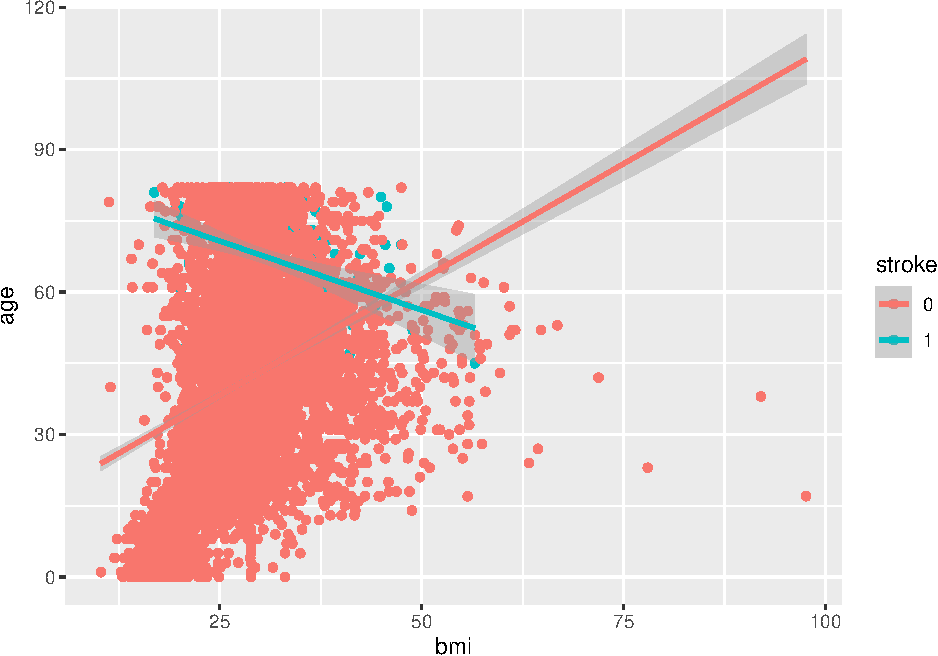
\includegraphics{sioux_mach_learn_project_files/figure-latex/unnamed-chunk-15-1.pdf}

\hypertarget{boxplots}{%
\subsection{Boxplots}\label{boxplots}}

With the following Boxplots the distribution of the data points is visualized. Again, not all Boxplots are included.

The following boxplot visualizes the distribution noStroke (0) and Stroke (1) by Age. As we can see the median Age for people suffering a Stroke is higher and is around 76 years old. Also the Distribution besides a few outliers is smaller.

\begin{Shaded}
\begin{Highlighting}[]
\NormalTok{stroke\_by\_age }\OtherTok{\textless{}{-}}\NormalTok{ stroke\_data }\SpecialCharTok{\%\textgreater{}\%}
\CommentTok{\# dplyr::filter(stroke == 1) \%\textgreater{}\%}
 \FunctionTok{ggplot}\NormalTok{(}\FunctionTok{aes}\NormalTok{(}\AttributeTok{x =}\NormalTok{ stroke,}
            \AttributeTok{y =}\NormalTok{ age)) }\SpecialCharTok{+}
  \FunctionTok{geom\_boxplot}\NormalTok{(}\AttributeTok{color=}\StringTok{"orange"}\NormalTok{, }\AttributeTok{fill=}\StringTok{"yellow"}\NormalTok{, }\AttributeTok{alpha=}\FloatTok{0.2}\NormalTok{) }\SpecialCharTok{+}
  \FunctionTok{ggtitle}\NormalTok{(}\StringTok{"Boxplot on no−Stroke (0) and Stroke (1) by Age"}\NormalTok{) }\SpecialCharTok{+} 
  \FunctionTok{xlab}\NormalTok{(}\StringTok{"Stroke"}\NormalTok{) }\SpecialCharTok{+} \FunctionTok{ylab}\NormalTok{(}\StringTok{"Age"}\NormalTok{) }\SpecialCharTok{+}
  \FunctionTok{theme\_minimal}\NormalTok{() }\SpecialCharTok{+} \FunctionTok{theme}\NormalTok{(}\AttributeTok{axis.text.x =} \FunctionTok{element\_text}\NormalTok{(}\AttributeTok{angle =} \DecValTok{0}\NormalTok{)) }
\NormalTok{stroke\_by\_age }
\end{Highlighting}
\end{Shaded}

\begin{verbatim}
## Warning in grid.Call(C_textBounds, as.graphicsAnnot(x$label), x$x, x$y, :
## conversion failure on 'Boxplot on no−Stroke (0) and Stroke (1) by Age' in
## 'mbcsToSbcs': dot substituted for <e2>
\end{verbatim}

\begin{verbatim}
## Warning in grid.Call(C_textBounds, as.graphicsAnnot(x$label), x$x, x$y, :
## conversion failure on 'Boxplot on no−Stroke (0) and Stroke (1) by Age' in
## 'mbcsToSbcs': dot substituted for <88>
\end{verbatim}

\begin{verbatim}
## Warning in grid.Call(C_textBounds, as.graphicsAnnot(x$label), x$x, x$y, :
## conversion failure on 'Boxplot on no−Stroke (0) and Stroke (1) by Age' in
## 'mbcsToSbcs': dot substituted for <92>
\end{verbatim}

\begin{verbatim}
## Warning in grid.Call(C_textBounds, as.graphicsAnnot(x$label), x$x, x$y, :
## conversion failure on 'Boxplot on no−Stroke (0) and Stroke (1) by Age' in
## 'mbcsToSbcs': dot substituted for <e2>
\end{verbatim}

\begin{verbatim}
## Warning in grid.Call(C_textBounds, as.graphicsAnnot(x$label), x$x, x$y, :
## conversion failure on 'Boxplot on no−Stroke (0) and Stroke (1) by Age' in
## 'mbcsToSbcs': dot substituted for <88>
\end{verbatim}

\begin{verbatim}
## Warning in grid.Call(C_textBounds, as.graphicsAnnot(x$label), x$x, x$y, :
## conversion failure on 'Boxplot on no−Stroke (0) and Stroke (1) by Age' in
## 'mbcsToSbcs': dot substituted for <92>
\end{verbatim}

\begin{verbatim}
## Warning in grid.Call(C_textBounds, as.graphicsAnnot(x$label), x$x, x$y, :
## conversion failure on 'Boxplot on no−Stroke (0) and Stroke (1) by Age' in
## 'mbcsToSbcs': dot substituted for <e2>
\end{verbatim}

\begin{verbatim}
## Warning in grid.Call(C_textBounds, as.graphicsAnnot(x$label), x$x, x$y, :
## conversion failure on 'Boxplot on no−Stroke (0) and Stroke (1) by Age' in
## 'mbcsToSbcs': dot substituted for <88>
\end{verbatim}

\begin{verbatim}
## Warning in grid.Call(C_textBounds, as.graphicsAnnot(x$label), x$x, x$y, :
## conversion failure on 'Boxplot on no−Stroke (0) and Stroke (1) by Age' in
## 'mbcsToSbcs': dot substituted for <92>
\end{verbatim}

\begin{verbatim}
## Warning in grid.Call(C_textBounds, as.graphicsAnnot(x$label), x$x, x$y, :
## conversion failure on 'Boxplot on no−Stroke (0) and Stroke (1) by Age' in
## 'mbcsToSbcs': dot substituted for <e2>
\end{verbatim}

\begin{verbatim}
## Warning in grid.Call(C_textBounds, as.graphicsAnnot(x$label), x$x, x$y, :
## conversion failure on 'Boxplot on no−Stroke (0) and Stroke (1) by Age' in
## 'mbcsToSbcs': dot substituted for <88>
\end{verbatim}

\begin{verbatim}
## Warning in grid.Call(C_textBounds, as.graphicsAnnot(x$label), x$x, x$y, :
## conversion failure on 'Boxplot on no−Stroke (0) and Stroke (1) by Age' in
## 'mbcsToSbcs': dot substituted for <92>
\end{verbatim}

\begin{verbatim}
## Warning in grid.Call(C_textBounds, as.graphicsAnnot(x$label), x$x, x$y, :
## conversion failure on 'Boxplot on no−Stroke (0) and Stroke (1) by Age' in
## 'mbcsToSbcs': dot substituted for <e2>
\end{verbatim}

\begin{verbatim}
## Warning in grid.Call(C_textBounds, as.graphicsAnnot(x$label), x$x, x$y, :
## conversion failure on 'Boxplot on no−Stroke (0) and Stroke (1) by Age' in
## 'mbcsToSbcs': dot substituted for <88>
\end{verbatim}

\begin{verbatim}
## Warning in grid.Call(C_textBounds, as.graphicsAnnot(x$label), x$x, x$y, :
## conversion failure on 'Boxplot on no−Stroke (0) and Stroke (1) by Age' in
## 'mbcsToSbcs': dot substituted for <92>
\end{verbatim}

\begin{verbatim}
## Warning in grid.Call(C_textBounds, as.graphicsAnnot(x$label), x$x, x$y, :
## conversion failure on 'Boxplot on no−Stroke (0) and Stroke (1) by Age' in
## 'mbcsToSbcs': dot substituted for <e2>
\end{verbatim}

\begin{verbatim}
## Warning in grid.Call(C_textBounds, as.graphicsAnnot(x$label), x$x, x$y, :
## conversion failure on 'Boxplot on no−Stroke (0) and Stroke (1) by Age' in
## 'mbcsToSbcs': dot substituted for <88>
\end{verbatim}

\begin{verbatim}
## Warning in grid.Call(C_textBounds, as.graphicsAnnot(x$label), x$x, x$y, :
## conversion failure on 'Boxplot on no−Stroke (0) and Stroke (1) by Age' in
## 'mbcsToSbcs': dot substituted for <92>
\end{verbatim}

\begin{verbatim}
## Warning in grid.Call(C_textBounds, as.graphicsAnnot(x$label), x$x, x$y, :
## conversion failure on 'Boxplot on no−Stroke (0) and Stroke (1) by Age' in
## 'mbcsToSbcs': dot substituted for <e2>
\end{verbatim}

\begin{verbatim}
## Warning in grid.Call(C_textBounds, as.graphicsAnnot(x$label), x$x, x$y, :
## conversion failure on 'Boxplot on no−Stroke (0) and Stroke (1) by Age' in
## 'mbcsToSbcs': dot substituted for <88>
\end{verbatim}

\begin{verbatim}
## Warning in grid.Call(C_textBounds, as.graphicsAnnot(x$label), x$x, x$y, :
## conversion failure on 'Boxplot on no−Stroke (0) and Stroke (1) by Age' in
## 'mbcsToSbcs': dot substituted for <92>
\end{verbatim}

\begin{verbatim}
## Warning in grid.Call.graphics(C_text, as.graphicsAnnot(x$label), x$x, x$y, :
## conversion failure on 'Boxplot on no−Stroke (0) and Stroke (1) by Age' in
## 'mbcsToSbcs': dot substituted for <e2>
\end{verbatim}

\begin{verbatim}
## Warning in grid.Call.graphics(C_text, as.graphicsAnnot(x$label), x$x, x$y, :
## conversion failure on 'Boxplot on no−Stroke (0) and Stroke (1) by Age' in
## 'mbcsToSbcs': dot substituted for <88>
\end{verbatim}

\begin{verbatim}
## Warning in grid.Call.graphics(C_text, as.graphicsAnnot(x$label), x$x, x$y, :
## conversion failure on 'Boxplot on no−Stroke (0) and Stroke (1) by Age' in
## 'mbcsToSbcs': dot substituted for <92>
\end{verbatim}

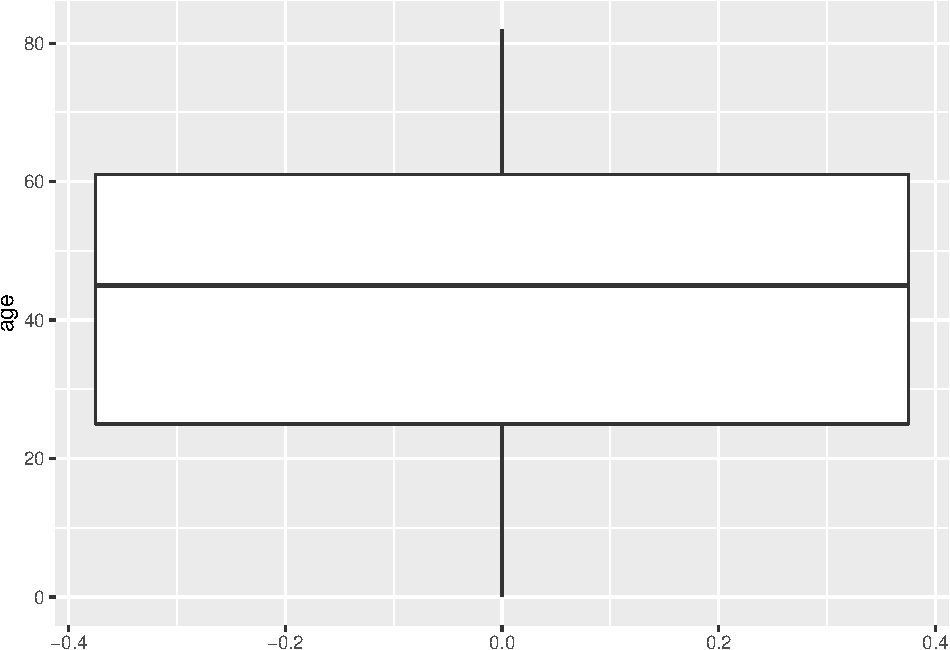
\includegraphics{sioux_mach_learn_project_files/figure-latex/unnamed-chunk-17-1.pdf}

In the following the distribution of the bmi by noStroke (0) and Stroke (1) is shown. As we can see the Median of the two variables are nearly the same around 26. For the people with noStroke (0) the distribution of the bmi is higher. There seems to be a lot of outliers with an high bmi.

\begin{Shaded}
\begin{Highlighting}[]
\NormalTok{stroke\_by\_bmi }\OtherTok{\textless{}{-}}\NormalTok{ stroke\_data }\SpecialCharTok{\%\textgreater{}\%}
\CommentTok{\# dplyr::filter(stroke == 1) \%\textgreater{}\%}
 \FunctionTok{ggplot}\NormalTok{(}\FunctionTok{aes}\NormalTok{(}\AttributeTok{x =}\NormalTok{ stroke,}
            \AttributeTok{y =}\NormalTok{ bmi)) }\SpecialCharTok{+}
  \FunctionTok{geom\_boxplot}\NormalTok{(}\AttributeTok{color=}\StringTok{"orange"}\NormalTok{, }\AttributeTok{fill=}\StringTok{"yellow"}\NormalTok{, }\AttributeTok{alpha=}\FloatTok{0.2}\NormalTok{) }\SpecialCharTok{+}
  \FunctionTok{ggtitle}\NormalTok{(}\StringTok{"BMI by Stroke"}\NormalTok{) }\SpecialCharTok{+} 
  \FunctionTok{xlab}\NormalTok{(}\StringTok{"Stroke"}\NormalTok{) }\SpecialCharTok{+} \FunctionTok{ylab}\NormalTok{(}\StringTok{"BMI"}\NormalTok{) }\SpecialCharTok{+}
  \FunctionTok{theme\_minimal}\NormalTok{() }\SpecialCharTok{+} \FunctionTok{theme}\NormalTok{(}\AttributeTok{axis.text.x =} \FunctionTok{element\_text}\NormalTok{(}\AttributeTok{angle =} \DecValTok{0}\NormalTok{))}
\NormalTok{stroke\_by\_bmi}
\end{Highlighting}
\end{Shaded}

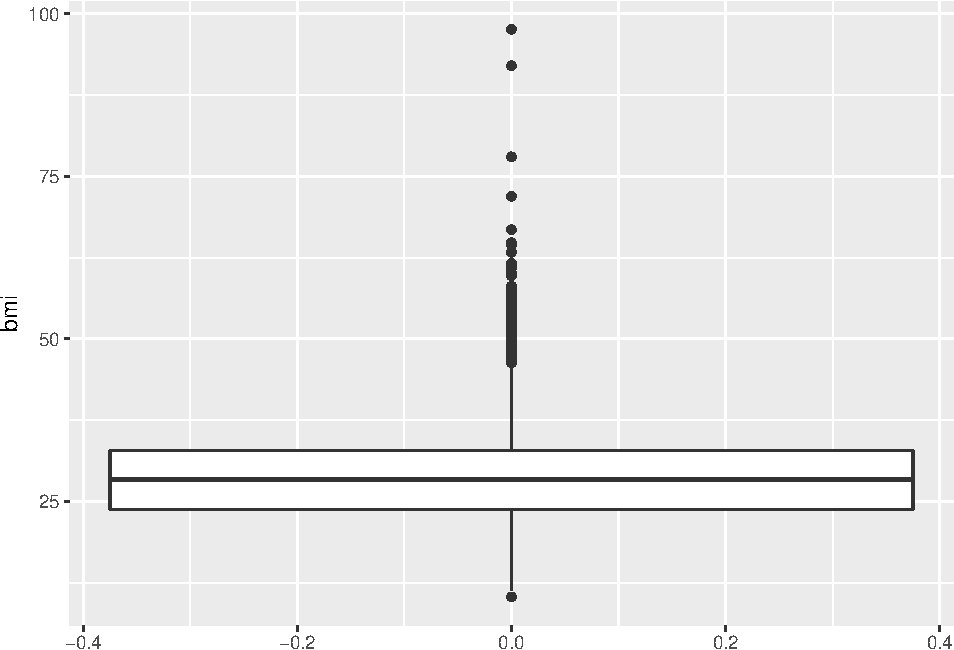
\includegraphics{sioux_mach_learn_project_files/figure-latex/unnamed-chunk-19-1.pdf}

\hypertarget{methodology}
\NormalTok{flag }\OtherTok{=} \FunctionTok{sort}\NormalTok{(}\FunctionTok{sample}\NormalTok{(}\DecValTok{1}\SpecialCharTok{:}\NormalTok{n, }\AttributeTok{size=}\NormalTok{n\_train, }\AttributeTok{replace=}\ConstantTok{FALSE}\NormalTok{))}
\end{Highlighting}
\end{Shaded}

\begin{verbatim}
## Warning in 1:n: numerical expression has 2 elements: only the first used
\end{verbatim}

\begin{Shaded}
\begin{Highlighting}[]
\CommentTok{\# Use df (all data points without ID column) df\_train, and df\_test}
\CommentTok{\# Gender, hypertension, heart disease, ever married, work type, residence type, smoking status, and stroke are all factor types.}
\CommentTok{\# This should allow for the best modeling options possible for our methods.}
\NormalTok{df\_train }\OtherTok{=}\NormalTok{ stroke\_data[flag,]}
\NormalTok{df\_test }\OtherTok{=}\NormalTok{ stroke\_data[}\SpecialCharTok{{-}}\NormalTok{flag,]}
\end{Highlighting}
\end{Shaded}

\begin{Shaded}
\begin{Highlighting}[]
\FunctionTok{head}\NormalTok{(df\_test)}
\end{Highlighting}
\end{Shaded}

\begin{verbatim}
## # A tibble: 6 x 13
##      id gender   age hypertension heart_disease ever_married work_type    
##   <dbl> <fct>  <int>        <dbl>         <dbl> <fct>        <fct>        
## 1 51676 Female    61            0             0 Yes          Self-employed
## 2 10434 Female    69            0             0 No           Private      
## 3 60491 Female    78            0             0 Yes          Private      
## 4 12095 Female    61            0             1 Yes          Govt_job     
## 5 58202 Female    50            1             0 Yes          Self-employed
## 6 56112 Male      64            0             1 Yes          Private      
## # ... with 6 more variables: residence_type <fct>, avg_glucose_level <dbl>,
## #   bmi <dbl>, smoking_status <fct>, stroke <fct>, stroke_num <dbl>
\end{verbatim}

\begin{Shaded}
\begin{Highlighting}[]
\FunctionTok{head}\NormalTok{(df\_train)}
\end{Highlighting}
\end{Shaded}

\begin{verbatim}
## # A tibble: 6 x 13
##      id gender   age hypertension heart_disease ever_married work_type    
##   <dbl> <fct>  <int>        <dbl>         <dbl> <fct>        <fct>        
## 1  9046 Male      67            0             1 Yes          Private      
## 2 31112 Male      80            0             1 Yes          Private      
## 3 60182 Female    49            0             0 Yes          Private      
## 4  1665 Female    79            1             0 Yes          Self-employed
## 5 56669 Male      81            0             0 Yes          Private      
## 6 53882 Male      74            1             1 Yes          Private      
## # ... with 6 more variables: residence_type <fct>, avg_glucose_level <dbl>,
## #   bmi <dbl>, smoking_status <fct>, stroke <fct>, stroke_num <dbl>
\end{verbatim}

\hypertarget{linear-models}
\NormalTok{flag }\OtherTok{=} \FunctionTok{sort}\NormalTok{(}\FunctionTok{sample}\NormalTok{(}\DecValTok{1}\SpecialCharTok{:}\NormalTok{n, }\AttributeTok{size=}\NormalTok{n\_train, }\AttributeTok{replace=}\ConstantTok{FALSE}\NormalTok{))}
\end{Highlighting}
\end{Shaded}

\begin{verbatim}
## Warning in 1:n: numerical expression has 2 elements: only the first used
\end{verbatim}

\begin{Shaded}
\begin{Highlighting}[]
\CommentTok{\# Use df (all data points without ID column) df\_train\_linear, and df\_test\_linear}
\CommentTok{\# Gender, hypertension, heart disease, ever married, work type, residence type, smoking status, and stroke are all factor types.}
\CommentTok{\# This should allow for the best modeling options possible for our methods.}
\NormalTok{df\_train\_linear }\OtherTok{=}\NormalTok{ stroke\_data[flag,]}
\NormalTok{df\_test\_linear }\OtherTok{=}\NormalTok{ stroke\_data[}\SpecialCharTok{{-}}\NormalTok{flag,]}
\end{Highlighting}
\end{Shaded}

\begin{Shaded}
\begin{Highlighting}[]
\FunctionTok{head}\NormalTok{(df\_test\_linear)}
\end{Highlighting}
\end{Shaded}

\begin{verbatim}
## # A tibble: 6 x 13
##      id gender   age hypertension heart_disease ever_married work_type    
##   <dbl> <fct>  <int>        <dbl>         <dbl> <fct>        <fct>        
## 1 51676 Female    61            0             0 Yes          Self-employed
## 2 10434 Female    69            0             0 No           Private      
## 3 60491 Female    78            0             0 Yes          Private      
## 4 12095 Female    61            0             1 Yes          Govt_job     
## 5 58202 Female    50            1             0 Yes          Self-employed
## 6 56112 Male      64            0             1 Yes          Private      
## # ... with 6 more variables: residence_type <fct>, avg_glucose_level <dbl>,
## #   bmi <dbl>, smoking_status <fct>, stroke <fct>, stroke_num <dbl>
\end{verbatim}

\begin{Shaded}
\begin{Highlighting}[]
\FunctionTok{head}\NormalTok{(df\_train\_linear)}
\end{Highlighting}
\end{Shaded}

\begin{verbatim}
## # A tibble: 6 x 13
##      id gender   age hypertension heart_disease ever_married work_type    
##   <dbl> <fct>  <int>        <dbl>         <dbl> <fct>        <fct>        
## 1  9046 Male      67            0             1 Yes          Private      
## 2 31112 Male      80            0             1 Yes          Private      
## 3 60182 Female    49            0             0 Yes          Private      
## 4  1665 Female    79            1             0 Yes          Self-employed
## 5 56669 Male      81            0             0 Yes          Private      
## 6 53882 Male      74            1             1 Yes          Private      
## # ... with 6 more variables: residence_type <fct>, avg_glucose_level <dbl>,
## #   bmi <dbl>, smoking_status <fct>, stroke <fct>, stroke_num <dbl>
\end{verbatim}

Our aim is to predict strokes, and the stroke variable is always our response variable of interest in this use case. However, simple or multiple linear regression is not the tool of choice, as stroke is a binary response variable.
Thus in the following we will nonetheless fit a linear regression model to our data with stroke as the response variable. However, out of all the linear methods, we will only focus on on a binomial model with family set to ``binomial'' in greater detail.

\hypertarget{selecting-predictors-for-the-model}{%
\subsection{Selecting Predictors for the model}\label{selecting-predictors-for-the-model}}

Apart from testing out individual variables, we also tested a model with all predictors to find out about the significant ones, as selecting all variables may not necessarily lead to a more accurate model, and we might run into overfitting problems. Furthermore, our variable selection is also informed by our exploratory plots above, and what we intuitively believe to be accurate risk factors for a stroke.

\begin{Shaded}
\begin{Highlighting}[]
\CommentTok{\# fitting models for simple regression model}
\NormalTok{lm.stroke.test }\OtherTok{\textless{}{-}} \FunctionTok{lm}\NormalTok{(stroke\_num }\SpecialCharTok{\textasciitilde{}}\NormalTok{ ., }\AttributeTok{data =}\NormalTok{ df\_train\_linear)}
\FunctionTok{summary}\NormalTok{(lm.stroke.test)}
\end{Highlighting}
\end{Shaded}

\begin{verbatim}
## Warning in summary.lm(lm.stroke.test): essentially perfect fit: summary may be
## unreliable
\end{verbatim}

\begin{verbatim}
## 
## Call:
## lm(formula = stroke_num ~ ., data = df_train_linear)
## 
## Residuals:
##        Min         1Q     Median         3Q        Max 
## -1.124e-15 -2.180e-18  4.000e-20  2.250e-18  9.299e-17 
## 
## Coefficients:
##                              Estimate Std. Error    t value Pr(>|t|)    
## (Intercept)                -4.797e-18  2.196e-18 -2.184e+00 0.029032 *  
## id                          1.498e-23  1.713e-23  8.740e-01 0.382064    
## genderMale                  4.919e-19  7.542e-19  6.520e-01 0.514290    
## genderOther                -3.276e-18  2.193e-17 -1.490e-01 0.881225    
## age                         3.668e-19  2.793e-20  1.313e+01  < 2e-16 ***
## hypertension                4.109e-18  1.265e-18  3.247e+00 0.001176 ** 
## heart_disease               7.985e-18  1.674e-18  4.771e+00 1.91e-06 ***
## ever_marriedYes            -4.324e-18  1.093e-18 -3.954e+00 7.83e-05 ***
## work_typeGovt_job          -7.648e-18  1.941e-18 -3.941e+00 8.27e-05 ***
## work_typeNever_worked      -3.312e-18  5.611e-18 -5.900e-01 0.555056    
## work_typePrivate           -5.647e-18  1.630e-18 -3.464e+00 0.000538 ***
## work_typeSelf-employed     -9.323e-18  1.981e-18 -4.705e+00 2.63e-06 ***
## residence_typeUrban         7.382e-20  7.327e-19  1.010e-01 0.919760    
## avg_glucose_level           3.220e-20  8.396e-21  3.835e+00 0.000128 ***
## bmi                        -5.681e-20  5.429e-20 -1.046e+00 0.295421    
## smoking_statusnever smoked -8.056e-19  1.086e-18 -7.420e-01 0.458274    
## smoking_statussmokes       -6.396e-19  1.295e-18 -4.940e-01 0.621509    
## smoking_statusUnknown      -1.744e-19  1.215e-18 -1.440e-01 0.885900    
## stroke1                     1.000e+00  1.751e-18  5.713e+17  < 2e-16 ***
## ---
## Signif. codes:  0 '***' 0.001 '**' 0.01 '*' 0.05 '.' 0.1 ' ' 1
## 
## Residual standard error: 2.187e-17 on 3558 degrees of freedom
## Multiple R-squared:      1,  Adjusted R-squared:      1 
## F-statistic: 2.006e+34 on 18 and 3558 DF,  p-value: < 2.2e-16
\end{verbatim}

Out of the significant predictors above, we chose the following model for the linear model, glm, and gam:

\begin{Shaded}
\begin{Highlighting}[]
\CommentTok{\# fitting models for simple regression model}
\NormalTok{linear\_model }\OtherTok{\textless{}{-}}\NormalTok{ stroke\_num }\SpecialCharTok{\textasciitilde{}}\NormalTok{ age }\SpecialCharTok{+}\NormalTok{ hypertension }\SpecialCharTok{+}\NormalTok{ heart\_disease }\SpecialCharTok{+}\NormalTok{ avg\_glucose\_level}
\end{Highlighting}
\end{Shaded}

Although ever married theoretically returns a significant result, this is most probably confounded by age, as can be seen in the plot below, the subjects that are or were married at some point tend to be significantly older than those that have never married.
The same is most likely true for the work type, with those having never worked being younger. What surprised us, though, is that smoking status did not have as big of an effect as we would have anticipated.

\begin{Shaded}
\begin{Highlighting}[]
\CommentTok{\# fitting models for simple regression model}
\NormalTok{lm.married }\OtherTok{\textless{}{-}} \FunctionTok{lm}\NormalTok{(age }\SpecialCharTok{\textasciitilde{}}\NormalTok{ ever\_married, }\AttributeTok{data =}\NormalTok{ df\_train\_linear)}
\FunctionTok{summary}\NormalTok{(lm.married)}
\end{Highlighting}
\end{Shaded}

\begin{verbatim}
## 
## Call:
## lm(formula = age ~ ever_married, data = df_train_linear)
## 
## Residuals:
##     Min      1Q  Median      3Q     Max 
## -36.575 -12.575  -1.575  10.425  59.838 
## 
## Coefficients:
##                 Estimate Std. Error t value Pr(>|t|)    
## (Intercept)      22.1622     0.4849   45.70   <2e-16 ***
## ever_marriedYes  32.4132     0.5944   54.53   <2e-16 ***
## ---
## Signif. codes:  0 '***' 0.001 '**' 0.01 '*' 0.05 '.' 0.1 ' ' 1
## 
## Residual standard error: 16.77 on 3575 degrees of freedom
## Multiple R-squared:  0.4541, Adjusted R-squared:  0.454 
## F-statistic:  2974 on 1 and 3575 DF,  p-value: < 2.2e-16
\end{verbatim}

\begin{Shaded}
\begin{Highlighting}[]
\FunctionTok{plot}\NormalTok{(age }\SpecialCharTok{\textasciitilde{}}\NormalTok{ ever\_married, }\AttributeTok{data =}\NormalTok{ df\_train\_linear)}
\FunctionTok{abline}\NormalTok{(lm.married)}
\end{Highlighting}
\end{Shaded}

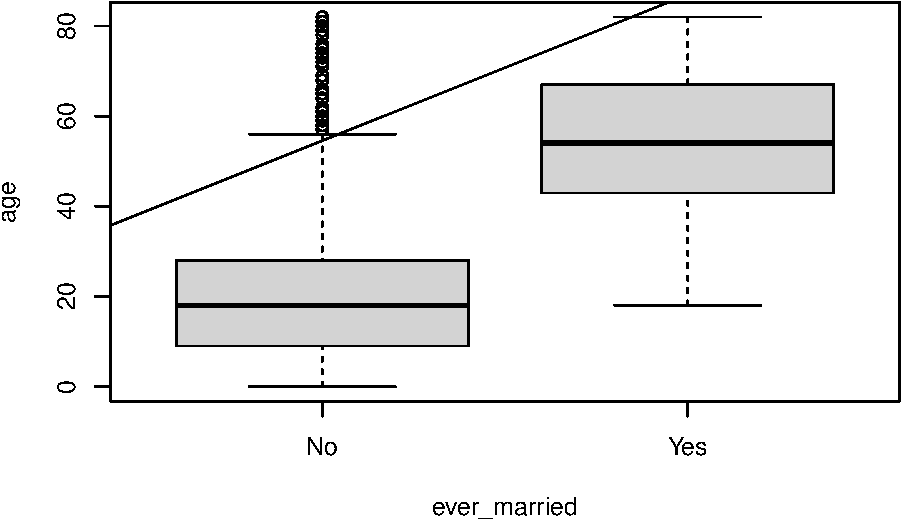
\includegraphics{sioux_mach_learn_project_files/figure-latex/unnamed-chunk-29-1.pdf}

\begin{Shaded}
\begin{Highlighting}[]
\CommentTok{\# fitting models for simple regression model}
\NormalTok{lm.stroke }\OtherTok{\textless{}{-}} \FunctionTok{lm}\NormalTok{(stroke\_num }\SpecialCharTok{\textasciitilde{}}\NormalTok{ age }\SpecialCharTok{+}\NormalTok{ hypertension }\SpecialCharTok{+}\NormalTok{ heart\_disease }\SpecialCharTok{*}\NormalTok{ avg\_glucose\_level, }\AttributeTok{data =}\NormalTok{ df\_train\_linear)}
\FunctionTok{summary}\NormalTok{(lm.stroke)}
\end{Highlighting}
\end{Shaded}

\begin{verbatim}
## 
## Call:
## lm(formula = stroke_num ~ age + hypertension + heart_disease * 
##     avg_glucose_level, data = df_train_linear)
## 
## Residuals:
##      Min       1Q   Median       3Q      Max 
## -0.36224 -0.07933 -0.03774  0.00549  1.05000 
## 
## Coefficients:
##                                   Estimate Std. Error t value Pr(>|t|)    
## (Intercept)                     -6.569e-02  1.080e-02  -6.084 1.29e-09 ***
## age                              1.977e-03  1.695e-04  11.663  < 2e-16 ***
## hypertension                     3.939e-02  1.203e-02   3.275  0.00107 ** 
## heart_disease                   -4.720e-02  3.679e-02  -1.283  0.19961    
## avg_glucose_level                1.949e-04  8.464e-05   2.302  0.02137 *  
## heart_disease:avg_glucose_level  9.962e-04  2.476e-04   4.024 5.84e-05 ***
## ---
## Signif. codes:  0 '***' 0.001 '**' 0.01 '*' 0.05 '.' 0.1 ' ' 1
## 
## Residual standard error: 0.2102 on 3571 degrees of freedom
## Multiple R-squared:  0.08625,    Adjusted R-squared:  0.08497 
## F-statistic: 67.42 on 5 and 3571 DF,  p-value: < 2.2e-16
\end{verbatim}

\begin{Shaded}
\begin{Highlighting}[]
\FunctionTok{plot}\NormalTok{(stroke\_num }\SpecialCharTok{\textasciitilde{}}\NormalTok{ age }\SpecialCharTok{+}\NormalTok{ hypertension }\SpecialCharTok{+}\NormalTok{ heart\_disease }\SpecialCharTok{+}\NormalTok{ avg\_glucose\_level, }\AttributeTok{data =}\NormalTok{ df\_train\_linear)}
\end{Highlighting}
\end{Shaded}

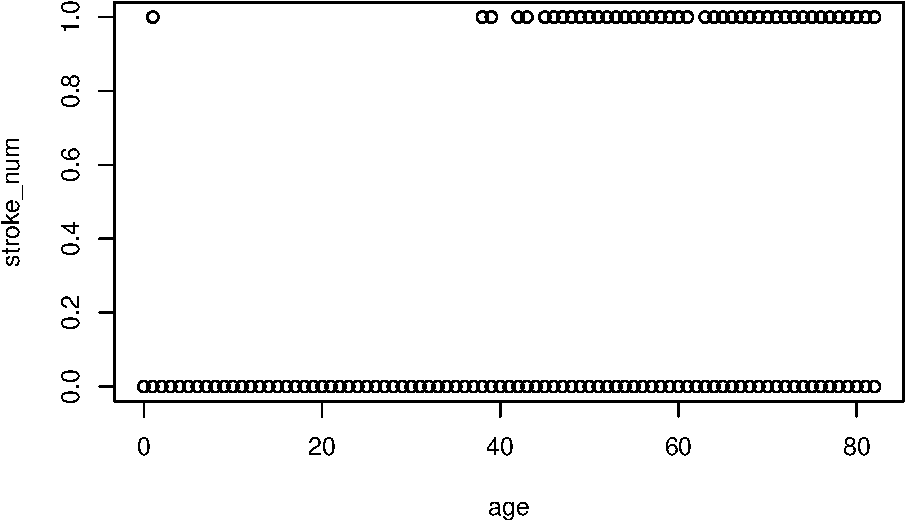
\includegraphics{sioux_mach_learn_project_files/figure-latex/unnamed-chunk-30-1.pdf} 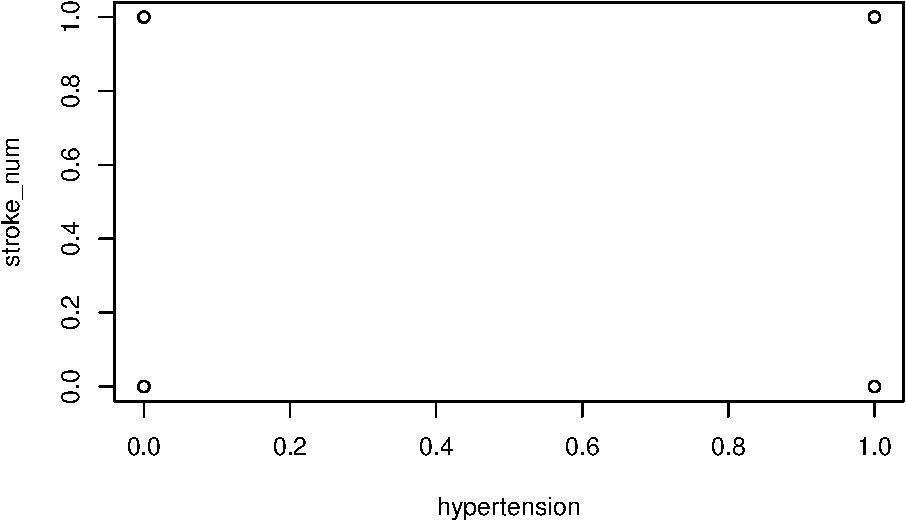
\includegraphics{sioux_mach_learn_project_files/figure-latex/unnamed-chunk-30-2.pdf} 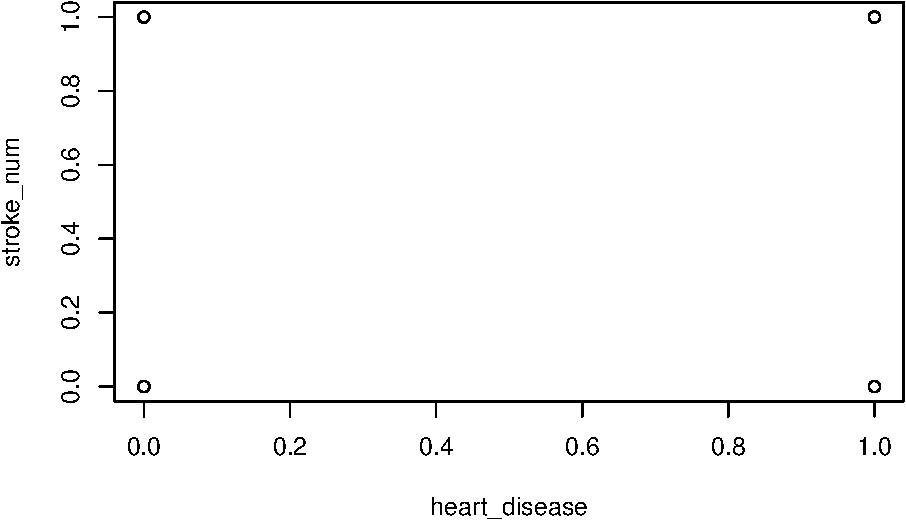
\includegraphics{sioux_mach_learn_project_files/figure-latex/unnamed-chunk-30-3.pdf}

\begin{Shaded}
\begin{Highlighting}[]
\FunctionTok{abline}\NormalTok{(lm.stroke)}
\end{Highlighting}
\end{Shaded}

\begin{verbatim}
## Warning in abline(lm.stroke): only using the first two of 6 regression
## coefficients
\end{verbatim}

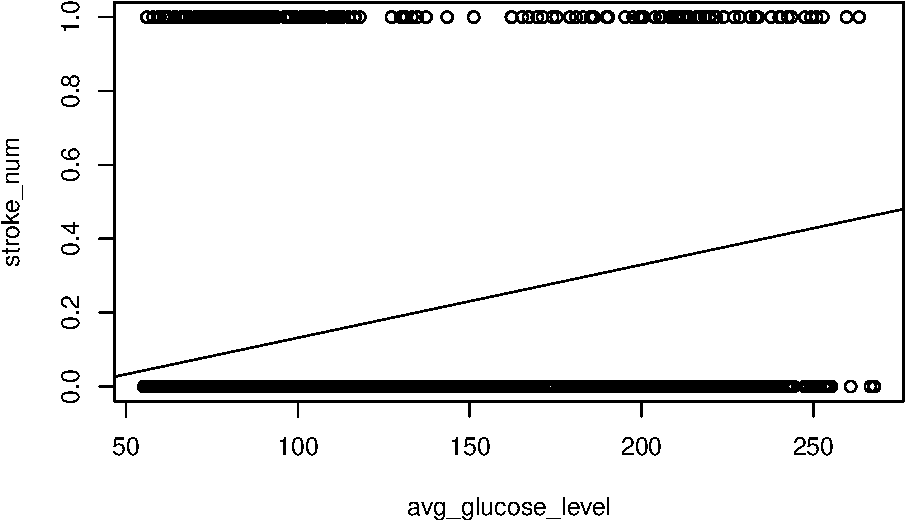
\includegraphics{sioux_mach_learn_project_files/figure-latex/unnamed-chunk-30-4.pdf}
Next, we evaluate the model fit with a confusion matrix. In the first example, we have constructed one ``manually''.
In all further examples we will be using the caret package's confusionMatrix() function.

\begin{Shaded}
\begin{Highlighting}[]
\CommentTok{\# Evaluating model fit using predict linear regression, example of a self{-}constructed confusion matrix}

\NormalTok{predicted.lm.stroke }\OtherTok{\textless{}{-}} \FunctionTok{ifelse}\NormalTok{(}\FunctionTok{predict}\NormalTok{(lm.stroke, df\_test\_linear, }\AttributeTok{type =} \StringTok{"response"}\NormalTok{) }\SpecialCharTok{\textless{}} \FloatTok{0.15}\NormalTok{, }\AttributeTok{yes =} \DecValTok{0}\NormalTok{, }\AttributeTok{no =} \DecValTok{1}\NormalTok{)}
\FunctionTok{head}\NormalTok{(predicted.lm.stroke)}
\end{Highlighting}
\end{Shaded}

\begin{verbatim}
## 1 2 3 4 5 6 
## 0 0 0 1 0 1
\end{verbatim}

\begin{Shaded}
\begin{Highlighting}[]
\NormalTok{obs.predicted.comp.lm }\OtherTok{\textless{}{-}} \FunctionTok{data.frame}\NormalTok{(}\AttributeTok{obs =}\NormalTok{ df\_test\_linear}\SpecialCharTok{$}\NormalTok{stroke\_num, }\AttributeTok{predicted =}\NormalTok{ predicted.lm.stroke)}

\FunctionTok{table}\NormalTok{(}\AttributeTok{obs =}\NormalTok{ obs.predicted.comp.lm}\SpecialCharTok{$}\NormalTok{obs, }\AttributeTok{fit =}\NormalTok{ obs.predicted.comp.lm}\SpecialCharTok{$}\NormalTok{predicted)}
\end{Highlighting}
\end{Shaded}

\begin{verbatim}
##    fit
## obs    0    1
##   0 1416   50
##   1   57   10
\end{verbatim}

\begin{Shaded}
\begin{Highlighting}[]
\FunctionTok{table}\NormalTok{(}\AttributeTok{obs =}\NormalTok{ obs.predicted.comp.lm}\SpecialCharTok{$}\NormalTok{obs, }\AttributeTok{fit =}\NormalTok{ obs.predicted.comp.lm}\SpecialCharTok{$}\NormalTok{predicted) }\SpecialCharTok{\%\textgreater{}\%}
  \FunctionTok{prop.table}\NormalTok{() }\SpecialCharTok{\%\textgreater{}\%}
  \FunctionTok{round}\NormalTok{(}\AttributeTok{digits =} \DecValTok{2}\NormalTok{)}
\end{Highlighting}
\end{Shaded}

\begin{verbatim}
##    fit
## obs    0    1
##   0 0.92 0.03
##   1 0.04 0.01
\end{verbatim}

\begin{Shaded}
\begin{Highlighting}[]
\CommentTok{\# Evaluating model fit using predict linear regression using confusionMatrix()}

\NormalTok{predicted.lm.stroke }\OtherTok{\textless{}{-}} \FunctionTok{ifelse}\NormalTok{(}\FunctionTok{predict}\NormalTok{(lm.stroke, df\_test\_linear, }\AttributeTok{type =} \StringTok{"response"}\NormalTok{) }\SpecialCharTok{\textless{}} \FloatTok{0.15}\NormalTok{, }\AttributeTok{yes =} \DecValTok{0}\NormalTok{, }\AttributeTok{no =} \DecValTok{1}\NormalTok{)}
\FunctionTok{head}\NormalTok{(predicted.lm.stroke)}
\end{Highlighting}
\end{Shaded}

\begin{verbatim}
## 1 2 3 4 5 6 
## 0 0 0 1 0 1
\end{verbatim}

\begin{Shaded}
\begin{Highlighting}[]
\FunctionTok{confusionMatrix}\NormalTok{(}\FunctionTok{as.factor}\NormalTok{(predicted.lm.stroke), }\FunctionTok{as.factor}\NormalTok{(df\_test\_linear}\SpecialCharTok{$}\NormalTok{stroke))}
\end{Highlighting}
\end{Shaded}

\begin{verbatim}
## Confusion Matrix and Statistics
## 
##           Reference
## Prediction    0    1
##          0 1416   57
##          1   50   10
##                                           
##                Accuracy : 0.9302          
##                  95% CI : (0.9163, 0.9424)
##     No Information Rate : 0.9563          
##     P-Value [Acc > NIR] : 1.0000          
##                                           
##                   Kappa : 0.1212          
##                                           
##  Mcnemar's Test P-Value : 0.5619          
##                                           
##             Sensitivity : 0.9659          
##             Specificity : 0.1493          
##          Pos Pred Value : 0.9613          
##          Neg Pred Value : 0.1667          
##              Prevalence : 0.9563          
##          Detection Rate : 0.9237          
##    Detection Prevalence : 0.9609          
##       Balanced Accuracy : 0.5576          
##                                           
##        'Positive' Class : 0               
## 
\end{verbatim}

\hypertarget{generalised-linear-model-with-family-set-to-poisson}{%
\section{Generalised Linear Model with family set to Poisson}\label{generalised-linear-model-with-family-set-to-poisson}}

\begin{Shaded}
\begin{Highlighting}[]
\CommentTok{\# text}
\NormalTok{glm.stroke.poisson }\OtherTok{\textless{}{-}} \FunctionTok{glm}\NormalTok{(stroke\_num }\SpecialCharTok{\textasciitilde{}}\NormalTok{ age }\SpecialCharTok{+}\NormalTok{ heart\_disease }\SpecialCharTok{+}\NormalTok{ hypertension }\SpecialCharTok{+}\NormalTok{ avg\_glucose\_level,}
\AttributeTok{family =} \StringTok{"poisson"}\NormalTok{,}
\AttributeTok{data =}\NormalTok{ df\_train\_linear)}
\FunctionTok{summary}\NormalTok{(glm.stroke.poisson)}
\end{Highlighting}
\end{Shaded}

\begin{verbatim}
## 
## Call:
## glm(formula = stroke_num ~ age + heart_disease + hypertension + 
##     avg_glucose_level, family = "poisson", data = df_train_linear)
## 
## Deviance Residuals: 
##     Min       1Q   Median       3Q      Max  
## -1.0558  -0.3142  -0.1712  -0.0831   3.4861  
## 
## Coefficients:
##                    Estimate Std. Error z value Pr(>|z|)    
## (Intercept)       -7.384780   0.413043 -17.879  < 2e-16 ***
## age                0.066499   0.005875  11.319  < 2e-16 ***
## heart_disease      0.356522   0.186276   1.914  0.05563 .  
## hypertension       0.296479   0.168541   1.759  0.07856 .  
## avg_glucose_level  0.003448   0.001222   2.823  0.00476 ** 
## ---
## Signif. codes:  0 '***' 0.001 '**' 0.01 '*' 0.05 '.' 0.1 ' ' 1
## 
## (Dispersion parameter for poisson family taken to be 1)
## 
##     Null deviance: 1084.09  on 3576  degrees of freedom
## Residual deviance:  795.51  on 3572  degrees of freedom
## AIC: 1169.5
## 
## Number of Fisher Scoring iterations: 7
\end{verbatim}

\begin{Shaded}
\begin{Highlighting}[]
\CommentTok{\#plot(stroke\_num \textasciitilde{} age + heart\_disease + hypertension + avg\_glucose\_level, data = df\_train\_linear)}
\CommentTok{\#abline(glm.stroke\_poisson)}
\FunctionTok{ggplot}\NormalTok{(}\AttributeTok{data =}\NormalTok{ df\_train\_linear, }\FunctionTok{aes}\NormalTok{(}\AttributeTok{x =}\NormalTok{ avg\_glucose\_level, }\AttributeTok{y =}\NormalTok{ stroke\_num)) }\SpecialCharTok{+} 
  \FunctionTok{geom\_jitter}\NormalTok{(}\AttributeTok{width =} \DecValTok{0}\NormalTok{, }\AttributeTok{height =} \FloatTok{0.05}\NormalTok{) }\SpecialCharTok{+}
  \FunctionTok{geom\_smooth}\NormalTok{(}\AttributeTok{method =} \StringTok{"glm"}\NormalTok{, }\AttributeTok{method.args =} \FunctionTok{list}\NormalTok{(}\AttributeTok{family =} \StringTok{"poisson"}\NormalTok{))}
\end{Highlighting}
\end{Shaded}

\begin{verbatim}
## `geom_smooth()` using formula 'y ~ x'
\end{verbatim}

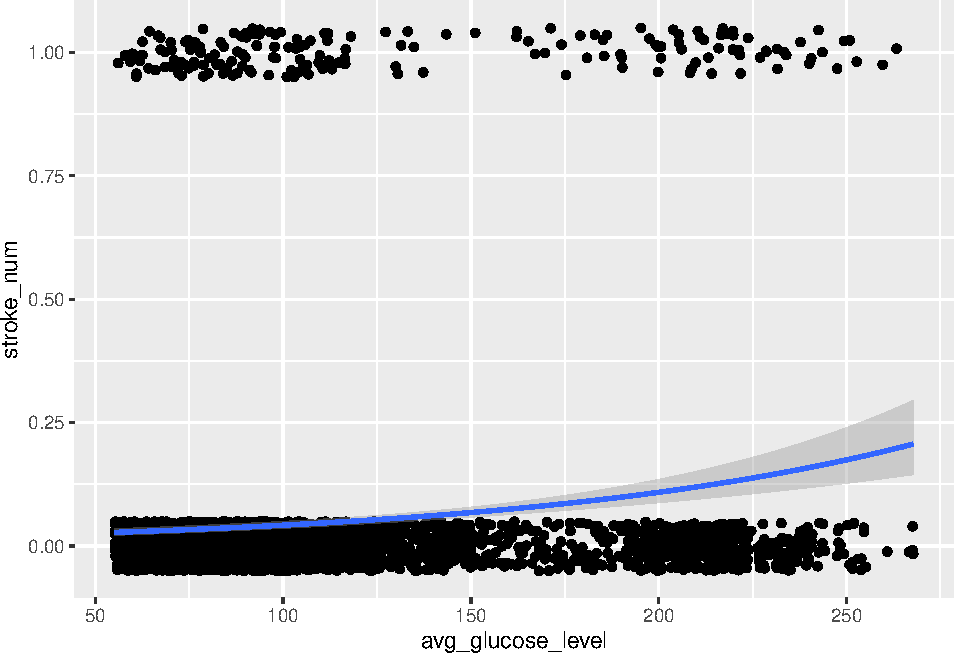
\includegraphics{sioux_mach_learn_project_files/figure-latex/unnamed-chunk-33-1.pdf}

Below is comparison of the fitted values versus the actual observed values within the training data set.

\begin{Shaded}
\begin{Highlighting}[]
\CommentTok{\# Evaluating model fit poisson}

\CommentTok{\# fitted(glm.stroke.poisson)}
\NormalTok{fitted.glm.stroke.poisson }\OtherTok{\textless{}{-}} \FunctionTok{ifelse}\NormalTok{(}\FunctionTok{fitted}\NormalTok{(glm.stroke.poisson) }\SpecialCharTok{\textless{}} \FloatTok{0.2}\NormalTok{, }\AttributeTok{yes =} \DecValTok{0}\NormalTok{, }\AttributeTok{no =} \DecValTok{1}\NormalTok{)}
\FunctionTok{head}\NormalTok{(fitted.glm.stroke.poisson)}
\end{Highlighting}
\end{Shaded}

\begin{verbatim}
## 1 2 3 4 5 6 
## 0 1 0 1 1 1
\end{verbatim}

\begin{Shaded}
\begin{Highlighting}[]
\NormalTok{obs.fitted.comp.poisson }\OtherTok{\textless{}{-}} \FunctionTok{data.frame}\NormalTok{(}\AttributeTok{obs =}\NormalTok{ df\_train\_linear}\SpecialCharTok{$}\NormalTok{stroke\_num, }\AttributeTok{fitted =}\NormalTok{ fitted.glm.stroke.poisson)}

\FunctionTok{table}\NormalTok{(}\AttributeTok{obs =}\NormalTok{ obs.fitted.comp.poisson}\SpecialCharTok{$}\NormalTok{obs, }\AttributeTok{fit =}\NormalTok{ obs.fitted.comp.poisson}\SpecialCharTok{$}\NormalTok{fitted)}
\end{Highlighting}
\end{Shaded}

\begin{verbatim}
##    fit
## obs    0    1
##   0 3238  157
##   1  130   52
\end{verbatim}

\begin{Shaded}
\begin{Highlighting}[]
\FunctionTok{table}\NormalTok{(}\AttributeTok{obs =}\NormalTok{ obs.fitted.comp.poisson}\SpecialCharTok{$}\NormalTok{obs, }\AttributeTok{fit =}\NormalTok{ obs.fitted.comp.poisson}\SpecialCharTok{$}\NormalTok{fitted) }\SpecialCharTok{\%\textgreater{}\%}
  \FunctionTok{prop.table}\NormalTok{() }\SpecialCharTok{\%\textgreater{}\%}
  \FunctionTok{round}\NormalTok{(}\AttributeTok{digits =} \DecValTok{2}\NormalTok{)}
\end{Highlighting}
\end{Shaded}

\begin{verbatim}
##    fit
## obs    0    1
##   0 0.91 0.04
##   1 0.04 0.01
\end{verbatim}

\begin{Shaded}
\begin{Highlighting}[]
\CommentTok{\# Evaluating model fit using predict linear regression using confusionMatrix()}

\NormalTok{glm.stroke.poisson.prediction }\OtherTok{\textless{}{-}} \FunctionTok{as.factor}\NormalTok{(}\FunctionTok{ifelse}\NormalTok{(}\FunctionTok{predict}\NormalTok{(glm.stroke.poisson, df\_test\_linear, }\AttributeTok{type =} \StringTok{"response"}\NormalTok{) }\SpecialCharTok{\textless{}} \FloatTok{0.15}\NormalTok{, }\AttributeTok{yes =} \DecValTok{0}\NormalTok{, }\AttributeTok{no =} \DecValTok{1}\NormalTok{))}
\FunctionTok{head}\NormalTok{(glm.stroke.poisson.prediction)}
\end{Highlighting}
\end{Shaded}

\begin{verbatim}
## 1 2 3 4 5 6 
## 0 0 0 0 0 0 
## Levels: 0 1
\end{verbatim}

\begin{Shaded}
\begin{Highlighting}[]
\FunctionTok{confusionMatrix}\NormalTok{(glm.stroke.poisson.prediction, df\_test\_linear}\SpecialCharTok{$}\NormalTok{stroke)}
\end{Highlighting}
\end{Shaded}

\begin{verbatim}
## Confusion Matrix and Statistics
## 
##           Reference
## Prediction    0    1
##          0 1355   46
##          1  111   21
##                                           
##                Accuracy : 0.8976          
##                  95% CI : (0.8813, 0.9123)
##     No Information Rate : 0.9563          
##     P-Value [Acc > NIR] : 1               
##                                           
##                   Kappa : 0.1625          
##                                           
##  Mcnemar's Test P-Value : 3.26e-07        
##                                           
##             Sensitivity : 0.9243          
##             Specificity : 0.3134          
##          Pos Pred Value : 0.9672          
##          Neg Pred Value : 0.1591          
##              Prevalence : 0.9563          
##          Detection Rate : 0.8839          
##    Detection Prevalence : 0.9139          
##       Balanced Accuracy : 0.6189          
##                                           
##        'Positive' Class : 0               
## 
\end{verbatim}

\hypertarget{generalised-linear-model-with-family-set-to-binomial}{%
\section{Generalised Linear Model with family set to Binomial}\label{generalised-linear-model-with-family-set-to-binomial}}

Since we are essentially dealing with a classification issue, using logistic regression in the form of a GLM with family set to ``binomial'' is the best method to apply out of all the models introduced so far. For this reason, we shall go into more detail here.

\begin{Shaded}
\begin{Highlighting}[]
\CommentTok{\# Include all variables to start variable selection}
\CommentTok{\# Plot all of them for visual analysis}
\NormalTok{glm.stroke.binomial }\OtherTok{\textless{}{-}} \FunctionTok{glm}\NormalTok{(stroke }\SpecialCharTok{\textasciitilde{}}\NormalTok{ age }\SpecialCharTok{+}\NormalTok{ gender }\SpecialCharTok{+}\NormalTok{ avg\_glucose\_level }\SpecialCharTok{+}\NormalTok{ residence\_type }\SpecialCharTok{+}\NormalTok{ work\_type }\SpecialCharTok{+}\NormalTok{ heart\_disease }\SpecialCharTok{+}\NormalTok{ hypertension }\SpecialCharTok{+}\NormalTok{ ever\_married }\SpecialCharTok{+}\NormalTok{ bmi }\SpecialCharTok{+}\NormalTok{ smoking\_status,}
\AttributeTok{family =} \StringTok{"binomial"}\NormalTok{,}
\AttributeTok{data =}\NormalTok{ df\_train\_linear)}
\FunctionTok{summary}\NormalTok{(glm.stroke.binomial)}
\end{Highlighting}
\end{Shaded}

\begin{verbatim}
## 
## Call:
## glm(formula = stroke ~ age + gender + avg_glucose_level + residence_type + 
##     work_type + heart_disease + hypertension + ever_married + 
##     bmi + smoking_status, family = "binomial", data = df_train_linear)
## 
## Deviance Residuals: 
##     Min       1Q   Median       3Q      Max  
## -1.3023  -0.3211  -0.1577  -0.0778   3.6948  
## 
## Coefficients:
##                              Estimate Std. Error z value Pr(>|z|)    
## (Intercept)                -7.320e+00  1.079e+00  -6.781 1.19e-11 ***
## age                         8.025e-02  7.152e-03  11.221  < 2e-16 ***
## genderMale                  1.941e-01  1.666e-01   1.165  0.24399    
## genderOther                -1.029e+01  1.455e+03  -0.007  0.99436    
## avg_glucose_level           3.678e-03  1.397e-03   2.632  0.00848 ** 
## residence_typeUrban        -2.994e-02  1.634e-01  -0.183  0.85465    
## work_typeGovt_job          -9.598e-01  1.139e+00  -0.843  0.39939    
## work_typeNever_worked      -1.015e+01  3.623e+02  -0.028  0.97766    
## work_typePrivate           -7.741e-01  1.122e+00  -0.690  0.49033    
## work_typeSelf-employed     -1.335e+00  1.145e+00  -1.166  0.24356    
## heart_disease               4.014e-01  2.150e-01   1.867  0.06191 .  
## hypertension                3.709e-01  1.903e-01   1.949  0.05132 .  
## ever_marriedYes            -2.280e-01  2.667e-01  -0.855  0.39271    
## bmi                         8.944e-03  1.338e-02   0.669  0.50380    
## smoking_statusnever smoked -1.636e-01  2.064e-01  -0.793  0.42796    
## smoking_statussmokes        4.783e-02  2.569e-01   0.186  0.85228    
## smoking_statusUnknown      -7.281e-02  2.442e-01  -0.298  0.76563    
## ---
## Signif. codes:  0 '***' 0.001 '**' 0.01 '*' 0.05 '.' 0.1 ' ' 1
## 
## (Dispersion parameter for binomial family taken to be 1)
## 
##     Null deviance: 1438.7  on 3576  degrees of freedom
## Residual deviance: 1115.1  on 3560  degrees of freedom
## AIC: 1149.1
## 
## Number of Fisher Scoring iterations: 14
\end{verbatim}

\begin{Shaded}
\begin{Highlighting}[]
\NormalTok{prediction.glm }\OtherTok{\textless{}{-}} \FunctionTok{predict}\NormalTok{(glm.stroke.binomial, df\_test\_linear, }\AttributeTok{type =} \StringTok{"response"}\NormalTok{)}
\CommentTok{\# InformationValue::optimalCutoff(df\_test\_linear, prediction.glm)}

\FunctionTok{str}\NormalTok{(prediction.glm)}
\end{Highlighting}
\end{Shaded}

\begin{verbatim}
##  Named num [1:1533] 0.0411 0.0998 0.1502 0.0839 0.0225 ...
##  - attr(*, "names")= chr [1:1533] "1" "2" "3" "4" ...
\end{verbatim}

\begin{Shaded}
\begin{Highlighting}[]
\NormalTok{predicted.glm.stroke.binomial }\OtherTok{\textless{}{-}} \FunctionTok{as.factor}\NormalTok{(}\FunctionTok{ifelse}\NormalTok{(}\FunctionTok{predict}\NormalTok{(glm.stroke.binomial, df\_test\_linear, }\AttributeTok{type =} \StringTok{"response"}\NormalTok{) }\SpecialCharTok{\textless{}} \FloatTok{0.15}\NormalTok{, }\AttributeTok{yes =} \DecValTok{0}\NormalTok{, }\AttributeTok{no =} \DecValTok{1}\NormalTok{))}
\FunctionTok{head}\NormalTok{(predicted.glm.stroke.binomial)}
\end{Highlighting}
\end{Shaded}

\begin{verbatim}
## 1 2 3 4 5 6 
## 0 0 1 0 0 1 
## Levels: 0 1
\end{verbatim}

\begin{Shaded}
\begin{Highlighting}[]
\FunctionTok{confusionMatrix}\NormalTok{(predicted.glm.stroke.binomial, df\_test\_linear}\SpecialCharTok{$}\NormalTok{stroke)}
\end{Highlighting}
\end{Shaded}

\begin{verbatim}
## Confusion Matrix and Statistics
## 
##           Reference
## Prediction    0    1
##          0 1351   44
##          1  115   23
##                                           
##                Accuracy : 0.8963          
##                  95% CI : (0.8799, 0.9111)
##     No Information Rate : 0.9563          
##     P-Value [Acc > NIR] : 1               
##                                           
##                   Kappa : 0.1759          
##                                           
##  Mcnemar's Test P-Value : 2.835e-08       
##                                           
##             Sensitivity : 0.9216          
##             Specificity : 0.3433          
##          Pos Pred Value : 0.9685          
##          Neg Pred Value : 0.1667          
##              Prevalence : 0.9563          
##          Detection Rate : 0.8813          
##    Detection Prevalence : 0.9100          
##       Balanced Accuracy : 0.6324          
##                                           
##        'Positive' Class : 0               
## 
\end{verbatim}

\begin{Shaded}
\begin{Highlighting}[]
\CommentTok{\# First iteration with parameters chosen from intuitive domain knowledge and exploratory analysis of data}
\NormalTok{glm.stroke.binomial }\OtherTok{\textless{}{-}} \FunctionTok{glm}\NormalTok{(stroke }\SpecialCharTok{\textasciitilde{}}\NormalTok{ age }\SpecialCharTok{+}\NormalTok{ heart\_disease }\SpecialCharTok{+}\NormalTok{ hypertension }\SpecialCharTok{+}\NormalTok{ work\_type }\SpecialCharTok{+}\NormalTok{ avg\_glucose\_level }\SpecialCharTok{+}\NormalTok{ smoking\_status,}
\AttributeTok{family =} \StringTok{"binomial"}\NormalTok{,}
\AttributeTok{data =}\NormalTok{ df\_train\_linear)}
\FunctionTok{summary}\NormalTok{(glm.stroke.binomial)}
\end{Highlighting}
\end{Shaded}

\begin{verbatim}
## 
## Call:
## glm(formula = stroke ~ age + heart_disease + hypertension + work_type + 
##     avg_glucose_level + smoking_status, family = "binomial", 
##     data = df_train_linear)
## 
## Deviance Residuals: 
##     Min       1Q   Median       3Q      Max  
## -1.1696  -0.3241  -0.1595  -0.0771   3.6785  
## 
## Coefficients:
##                              Estimate Std. Error z value Pr(>|z|)    
## (Intercept)                 -7.037953   1.036288  -6.792 1.11e-11 ***
## age                          0.078346   0.006958  11.260  < 2e-16 ***
## heart_disease                0.431469   0.213875   2.017   0.0437 *  
## hypertension                 0.378996   0.189527   2.000   0.0455 *  
## work_typeGovt_job           -1.003706   1.105068  -0.908   0.3637    
## work_typeNever_worked      -10.077332 362.934034  -0.028   0.9778    
## work_typePrivate            -0.818567   1.088363  -0.752   0.4520    
## work_typeSelf-employed      -1.382649   1.112789  -1.243   0.2140    
## avg_glucose_level            0.003936   0.001360   2.894   0.0038 ** 
## smoking_statusnever smoked  -0.186796   0.203452  -0.918   0.3586    
## smoking_statussmokes         0.032194   0.256225   0.126   0.9000    
## smoking_statusUnknown       -0.081986   0.243356  -0.337   0.7362    
## ---
## Signif. codes:  0 '***' 0.001 '**' 0.01 '*' 0.05 '.' 0.1 ' ' 1
## 
## (Dispersion parameter for binomial family taken to be 1)
## 
##     Null deviance: 1438.7  on 3576  degrees of freedom
## Residual deviance: 1117.5  on 3565  degrees of freedom
## AIC: 1141.5
## 
## Number of Fisher Scoring iterations: 14
\end{verbatim}

\begin{Shaded}
\begin{Highlighting}[]
\CommentTok{\#plot(stroke \textasciitilde{} age + heart\_disease + hypertension + work\_type + avg\_glucose\_level + smoking\_status, data = df\_train\_linear)}
\CommentTok{\#abline(glm.stroke.binomial)}
\end{Highlighting}
\end{Shaded}

\begin{Shaded}
\begin{Highlighting}[]
\CommentTok{\# second iteration only keeping statistically relevant parameters from previous model}
\NormalTok{glm.stroke.binomial}\FloatTok{.2} \OtherTok{\textless{}{-}} \FunctionTok{glm}\NormalTok{(stroke\_num }\SpecialCharTok{\textasciitilde{}}\NormalTok{ age }\SpecialCharTok{+}\NormalTok{ heart\_disease }\SpecialCharTok{+}\NormalTok{ hypertension }\SpecialCharTok{+}\NormalTok{ avg\_glucose\_level,}
\AttributeTok{family =} \StringTok{"binomial"}\NormalTok{,}
\AttributeTok{data =}\NormalTok{ df\_train\_linear)}
\FunctionTok{summary}\NormalTok{(glm.stroke.binomial}\FloatTok{.2}\NormalTok{)}
\end{Highlighting}
\end{Shaded}

\begin{verbatim}
## 
## Call:
## glm(formula = stroke_num ~ age + heart_disease + hypertension + 
##     avg_glucose_level, family = "binomial", data = df_train_linear)
## 
## Deviance Residuals: 
##     Min       1Q   Median       3Q      Max  
## -1.1183  -0.3237  -0.1671  -0.0764   3.8413  
## 
## Coefficients:
##                    Estimate Std. Error z value Pr(>|z|)    
## (Intercept)       -7.739236   0.443953 -17.433   <2e-16 ***
## age                0.072374   0.006312  11.467   <2e-16 ***
## heart_disease      0.465121   0.211312   2.201   0.0277 *  
## hypertension       0.362843   0.187103   1.939   0.0525 .  
## avg_glucose_level  0.004117   0.001351   3.048   0.0023 ** 
## ---
## Signif. codes:  0 '***' 0.001 '**' 0.01 '*' 0.05 '.' 0.1 ' ' 1
## 
## (Dispersion parameter for binomial family taken to be 1)
## 
##     Null deviance: 1438.7  on 3576  degrees of freedom
## Residual deviance: 1127.6  on 3572  degrees of freedom
## AIC: 1137.6
## 
## Number of Fisher Scoring iterations: 7
\end{verbatim}

\begin{Shaded}
\begin{Highlighting}[]
\CommentTok{\# plot(stroke \textasciitilde{} age + heart\_disease + hypertension + avg\_glucose\_level, data = df\_train\_linear)}
\CommentTok{\# abline(glm.stroke.binomial.2)}

\NormalTok{pred }\OtherTok{\textless{}{-}} \FunctionTok{predict}\NormalTok{(glm.stroke.binomial}\FloatTok{.2}\NormalTok{)}
\CommentTok{\# pred}

\FunctionTok{ggplot}\NormalTok{(}\AttributeTok{data =}\NormalTok{ df\_train\_linear, }\FunctionTok{aes}\NormalTok{(}\AttributeTok{x =}\NormalTok{ age, }\AttributeTok{y =}\NormalTok{ stroke\_num)) }\SpecialCharTok{+} 
  \FunctionTok{geom\_jitter}\NormalTok{(}\AttributeTok{width =} \DecValTok{0}\NormalTok{, }\AttributeTok{height =} \FloatTok{0.05}\NormalTok{) }\SpecialCharTok{+}
  \FunctionTok{geom\_smooth}\NormalTok{(}\AttributeTok{method =} \StringTok{"glm"}\NormalTok{, }\AttributeTok{method.args =} \FunctionTok{list}\NormalTok{(}\AttributeTok{family =} \StringTok{"binomial"}\NormalTok{))}
\end{Highlighting}
\end{Shaded}

\begin{verbatim}
## `geom_smooth()` using formula 'y ~ x'
\end{verbatim}

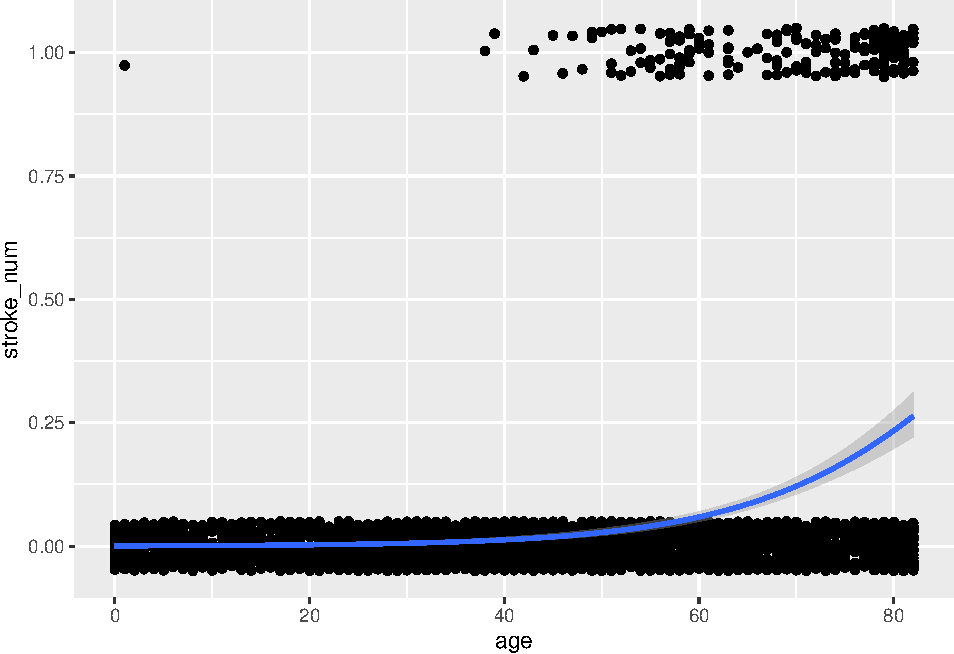
\includegraphics{sioux_mach_learn_project_files/figure-latex/unnamed-chunk-40-1.pdf}

\begin{Shaded}
\begin{Highlighting}[]
\NormalTok{predicted.glm.stroke.binomial}\FloatTok{.2} \OtherTok{\textless{}{-}} \FunctionTok{as.factor}\NormalTok{(}\FunctionTok{ifelse}\NormalTok{(}\FunctionTok{predict}\NormalTok{(glm.stroke.binomial}\FloatTok{.2}\NormalTok{, df\_test\_linear, }\AttributeTok{type =} \StringTok{"response"}\NormalTok{) }\SpecialCharTok{\textless{}} \FloatTok{0.2}\NormalTok{, }\AttributeTok{yes =} \DecValTok{0}\NormalTok{, }\AttributeTok{no =} \DecValTok{1}\NormalTok{))}
\FunctionTok{head}\NormalTok{(predicted.glm.stroke.binomial}\FloatTok{.2}\NormalTok{)}
\end{Highlighting}
\end{Shaded}

\begin{verbatim}
## 1 2 3 4 5 6 
## 0 0 0 0 0 0 
## Levels: 0 1
\end{verbatim}

\begin{Shaded}
\begin{Highlighting}[]
\CommentTok{\# predicted.glm.stroke.binomial.2 \textless{}{-} as.factor(predicted.glm.stroke.binomial.2)}
\CommentTok{\# predicted.glm.stroke.binomial.2 \textless{}{-} relevel(predicted.glm.stroke.binomial.2, "0")}

\FunctionTok{confusionMatrix}\NormalTok{(predicted.glm.stroke.binomial}\FloatTok{.2}\NormalTok{, df\_test\_linear}\SpecialCharTok{$}\NormalTok{stroke)}
\end{Highlighting}
\end{Shaded}

\begin{verbatim}
## Confusion Matrix and Statistics
## 
##           Reference
## Prediction    0    1
##          0 1412   54
##          1   54   13
##                                           
##                Accuracy : 0.9295          
##                  95% CI : (0.9156, 0.9419)
##     No Information Rate : 0.9563          
##     P-Value [Acc > NIR] : 1               
##                                           
##                   Kappa : 0.1572          
##                                           
##  Mcnemar's Test P-Value : 1               
##                                           
##             Sensitivity : 0.9632          
##             Specificity : 0.1940          
##          Pos Pred Value : 0.9632          
##          Neg Pred Value : 0.1940          
##              Prevalence : 0.9563          
##          Detection Rate : 0.9211          
##    Detection Prevalence : 0.9563          
##       Balanced Accuracy : 0.5786          
##                                           
##        'Positive' Class : 0               
## 
\end{verbatim}

\hypertarget{generalised-additive-model}{%
\section{Generalised Additive Model}\label{generalised-additive-model}}

\begin{Shaded}
\begin{Highlighting}[]
\FunctionTok{library}\NormalTok{(mgcv)}

\NormalTok{gam.stroke }\OtherTok{\textless{}{-}} \FunctionTok{gam}\NormalTok{(stroke\_num }\SpecialCharTok{\textasciitilde{}}\NormalTok{ age }\SpecialCharTok{+}\NormalTok{ heart\_disease }\SpecialCharTok{+}\NormalTok{ hypertension }\SpecialCharTok{+}\NormalTok{ avg\_glucose\_level,}
\AttributeTok{family =} \StringTok{"binomial"}\NormalTok{,}
\AttributeTok{data =}\NormalTok{ df\_train\_linear)}
\FunctionTok{summary}\NormalTok{(gam.stroke)}
\end{Highlighting}
\end{Shaded}

\begin{verbatim}
## 
## Family: binomial 
## Link function: logit 
## 
## Formula:
## stroke_num ~ age + heart_disease + hypertension + avg_glucose_level
## 
## Parametric coefficients:
##                    Estimate Std. Error z value Pr(>|z|)    
## (Intercept)       -7.739236   0.443974 -17.432   <2e-16 ***
## age                0.072374   0.006312  11.466   <2e-16 ***
## heart_disease      0.465121   0.211313   2.201   0.0277 *  
## hypertension       0.362843   0.187105   1.939   0.0525 .  
## avg_glucose_level  0.004117   0.001351   3.048   0.0023 ** 
## ---
## Signif. codes:  0 '***' 0.001 '**' 0.01 '*' 0.05 '.' 0.1 ' ' 1
## 
## 
## R-sq.(adj) =  0.101   Deviance explained = 21.6%
## UBRE = -0.68197  Scale est. = 1         n = 3577
\end{verbatim}

\begin{Shaded}
\begin{Highlighting}[]
\CommentTok{\#plot(stroke \textasciitilde{} smoking\_status, data = df\_train\_linear)}
\CommentTok{\#abline(gam.stroke)}
\end{Highlighting}
\end{Shaded}

\begin{Shaded}
\begin{Highlighting}[]
\NormalTok{predicted.gam.stroke }\OtherTok{\textless{}{-}} \FunctionTok{as.factor}\NormalTok{(}\FunctionTok{ifelse}\NormalTok{(}\FunctionTok{predict}\NormalTok{( gam.stroke, df\_test\_linear, }\AttributeTok{type =} \StringTok{"response"}\NormalTok{) }\SpecialCharTok{\textless{}} \FloatTok{0.2}\NormalTok{, }\AttributeTok{yes =} \DecValTok{0}\NormalTok{, }\AttributeTok{no =} \DecValTok{1}\NormalTok{))}
\FunctionTok{head}\NormalTok{(predicted.gam.stroke)}
\end{Highlighting}
\end{Shaded}

\begin{verbatim}
## 1 2 3 4 5 6 
## 0 0 0 0 0 0 
## Levels: 0 1
\end{verbatim}

\begin{Shaded}
\begin{Highlighting}[]
\FunctionTok{confusionMatrix}\NormalTok{(predicted.gam.stroke, df\_test\_linear}\SpecialCharTok{$}\NormalTok{stroke)}
\end{Highlighting}
\end{Shaded}

\begin{verbatim}
## Confusion Matrix and Statistics
## 
##           Reference
## Prediction    0    1
##          0 1412   54
##          1   54   13
##                                           
##                Accuracy : 0.9295          
##                  95% CI : (0.9156, 0.9419)
##     No Information Rate : 0.9563          
##     P-Value [Acc > NIR] : 1               
##                                           
##                   Kappa : 0.1572          
##                                           
##  Mcnemar's Test P-Value : 1               
##                                           
##             Sensitivity : 0.9632          
##             Specificity : 0.1940          
##          Pos Pred Value : 0.9632          
##          Neg Pred Value : 0.1940          
##              Prevalence : 0.9563          
##          Detection Rate : 0.9211          
##    Detection Prevalence : 0.9563          
##       Balanced Accuracy : 0.5786          
##                                           
##        'Positive' Class : 0               
## 
\end{verbatim}

\hypertarget{neural-network-yves}{%
\section{Neural Network Yves}\label{neural-network-yves}}

\begin{Shaded}
\begin{Highlighting}[]
\CommentTok{\# read the csv agein, because the data needs to be idfferently prepared than in other model}
\NormalTok{stroke\_data\_nn }\OtherTok{\textless{}{-}} \FunctionTok{read\_csv}\NormalTok{(}\StringTok{\textquotesingle{}./data/healthcare{-}dataset{-}stroke{-}data.csv\textquotesingle{}}\NormalTok{)}
\end{Highlighting}
\end{Shaded}

\begin{verbatim}
## Rows: 5110 Columns: 12
## -- Column specification --------------------------------------------------------
## Delimiter: ","
## chr (6): gender, ever_married, work_type, Residence_type, bmi, smoking_status
## dbl (6): id, age, hypertension, heart_disease, avg_glucose_level, stroke
## 
## i Use `spec()` to retrieve the full column specification for this data.
## i Specify the column types or set `show_col_types = FALSE` to quiet this message.
\end{verbatim}

\begin{Shaded}
\begin{Highlighting}[]
\CommentTok{\# have a look at the data {-}\textgreater{} it is discovered, that bmi is not numeric, let\textquotesingle{}s change that}
\FunctionTok{str}\NormalTok{(stroke\_data\_nn)}
\end{Highlighting}
\end{Shaded}

\begin{verbatim}
## spec_tbl_df [5,110 x 12] (S3: spec_tbl_df/tbl_df/tbl/data.frame)
##  $ id               : num [1:5110] 9046 51676 31112 60182 1665 ...
##  $ gender           : chr [1:5110] "Male" "Female" "Male" "Female" ...
##  $ age              : num [1:5110] 67 61 80 49 79 81 74 69 59 78 ...
##  $ hypertension     : num [1:5110] 0 0 0 0 1 0 1 0 0 0 ...
##  $ heart_disease    : num [1:5110] 1 0 1 0 0 0 1 0 0 0 ...
##  $ ever_married     : chr [1:5110] "Yes" "Yes" "Yes" "Yes" ...
##  $ work_type        : chr [1:5110] "Private" "Self-employed" "Private" "Private" ...
##  $ Residence_type   : chr [1:5110] "Urban" "Rural" "Rural" "Urban" ...
##  $ avg_glucose_level: num [1:5110] 229 202 106 171 174 ...
##  $ bmi              : chr [1:5110] "36.6" "N/A" "32.5" "34.4" ...
##  $ smoking_status   : chr [1:5110] "formerly smoked" "never smoked" "never smoked" "smokes" ...
##  $ stroke           : num [1:5110] 1 1 1 1 1 1 1 1 1 1 ...
##  - attr(*, "spec")=
##   .. cols(
##   ..   id = col_double(),
##   ..   gender = col_character(),
##   ..   age = col_double(),
##   ..   hypertension = col_double(),
##   ..   heart_disease = col_double(),
##   ..   ever_married = col_character(),
##   ..   work_type = col_character(),
##   ..   Residence_type = col_character(),
##   ..   avg_glucose_level = col_double(),
##   ..   bmi = col_character(),
##   ..   smoking_status = col_character(),
##   ..   stroke = col_double()
##   .. )
##  - attr(*, "problems")=<externalptr>
\end{verbatim}

\begin{Shaded}
\begin{Highlighting}[]
\NormalTok{stroke\_data\_nn[}\DecValTok{10}\NormalTok{] }\OtherTok{\textless{}{-}} \FunctionTok{sapply}\NormalTok{(stroke\_data\_nn[}\DecValTok{10}\NormalTok{], as.numeric)}
\end{Highlighting}
\end{Shaded}

\begin{verbatim}
## Warning in lapply(X = X, FUN = FUN, ...): NAs introduced by coercion
\end{verbatim}

\begin{Shaded}
\begin{Highlighting}[]
\FunctionTok{str}\NormalTok{(stroke\_data\_nn)}
\end{Highlighting}
\end{Shaded}

\begin{verbatim}
## spec_tbl_df [5,110 x 12] (S3: spec_tbl_df/tbl_df/tbl/data.frame)
##  $ id               : num [1:5110] 9046 51676 31112 60182 1665 ...
##  $ gender           : chr [1:5110] "Male" "Female" "Male" "Female" ...
##  $ age              : num [1:5110] 67 61 80 49 79 81 74 69 59 78 ...
##  $ hypertension     : num [1:5110] 0 0 0 0 1 0 1 0 0 0 ...
##  $ heart_disease    : num [1:5110] 1 0 1 0 0 0 1 0 0 0 ...
##  $ ever_married     : chr [1:5110] "Yes" "Yes" "Yes" "Yes" ...
##  $ work_type        : chr [1:5110] "Private" "Self-employed" "Private" "Private" ...
##  $ Residence_type   : chr [1:5110] "Urban" "Rural" "Rural" "Urban" ...
##  $ avg_glucose_level: num [1:5110] 229 202 106 171 174 ...
##  $ bmi              : num [1:5110] 36.6 NA 32.5 34.4 24 29 27.4 22.8 NA 24.2 ...
##  $ smoking_status   : chr [1:5110] "formerly smoked" "never smoked" "never smoked" "smokes" ...
##  $ stroke           : num [1:5110] 1 1 1 1 1 1 1 1 1 1 ...
##  - attr(*, "spec")=
##   .. cols(
##   ..   id = col_double(),
##   ..   gender = col_character(),
##   ..   age = col_double(),
##   ..   hypertension = col_double(),
##   ..   heart_disease = col_double(),
##   ..   ever_married = col_character(),
##   ..   work_type = col_character(),
##   ..   Residence_type = col_character(),
##   ..   avg_glucose_level = col_double(),
##   ..   bmi = col_character(),
##   ..   smoking_status = col_character(),
##   ..   stroke = col_double()
##   .. )
##  - attr(*, "problems")=<externalptr>
\end{verbatim}

\begin{Shaded}
\begin{Highlighting}[]
\CommentTok{\#install.packages("caret")}
\end{Highlighting}
\end{Shaded}

\begin{Shaded}
\begin{Highlighting}[]
\CommentTok{\# make a df with only numeric values}
\CommentTok{\#numeric\_var\_original\_scale \textless{}{-} stroke\_data\_nn \%\textgreater{}\% select(where(is.numeric) \& !where(is.integer))}

\CommentTok{\#cat\_var \textless{}{-} stroke\_data\_nn[,!(names(stroke\_data\_nn) \%in\% names(numeric\_var\_original\_scale))] \%\textgreater{}\% select({-}stroke)}

\CommentTok{\#target\_var= (stroke\_data\_nn \%\textgreater{}\% select(stroke)) \%\textgreater{}\% }
\CommentTok{\#  mutate(stroke=as.factor(ifelse(stroke==0, "no\_stroke","stroke" )))}
\end{Highlighting}
\end{Shaded}

\begin{Shaded}
\begin{Highlighting}[]
\CommentTok{\# have a look at the structure of each df}
\CommentTok{\#str(numeric\_var)}
\CommentTok{\#str(cat\_var)}
\CommentTok{\#str(target\_var)}
\end{Highlighting}
\end{Shaded}

\begin{Shaded}
\begin{Highlighting}[]
\CommentTok{\#get parameters of center scale to use in train and unseen data with caret library}

\CommentTok{\#library(caret)}

\CommentTok{\#preproc.param\_comp \textless{}{-} numeric\_var\_original\_scale  \%\textgreater{}\% preProcess(method = c("center", "scale"))}

\CommentTok{\#numeric\_var \textless{}{-} preproc.param\_comp \%\textgreater{}\% predict(numeric\_var\_original\_scale)}

\CommentTok{\#predictors\_var= cbind.data.frame(cat\_var,numeric\_var)}
\end{Highlighting}
\end{Shaded}

\begin{Shaded}
\begin{Highlighting}[]
\CommentTok{\#now we have:}
\CommentTok{\#head(target\_var)}
\end{Highlighting}
\end{Shaded}

\begin{Shaded}
\begin{Highlighting}[]
\CommentTok{\#NA values are already solved, so lets see if some predictors have small variances:}
\CommentTok{\# Identify near zero variance predictors: remove\_cols}

\CommentTok{\#remove\_cols \textless{}{-} nearZeroVar(numeric\_var, names = TRUE, }
\CommentTok{\#                           freqCut = 10, uniqueCut = 20)}

\CommentTok{\#remove\_cols}
\end{Highlighting}
\end{Shaded}

\begin{Shaded}
\begin{Highlighting}[]
\CommentTok{\#lets see if some predictor have some high leverage point}
\CommentTok{\#plot(numeric\_var)}
\end{Highlighting}
\end{Shaded}

\begin{Shaded}
\begin{Highlighting}[]
\CommentTok{\#it\textquotesingle{}s ok for me, lets see correlation between variables matrix}
\CommentTok{\#numeric\_varcor = numeric\_var\_original\_scale}
\CommentTok{\#names(numeric\_varcor) = c("Age", "Avg. glucose level", "BMI")}

\CommentTok{\#correlationMatrix1 \textless{}{-} round(cor(numeric\_varcor),2) }
\end{Highlighting}
\end{Shaded}

\begin{Shaded}
\begin{Highlighting}[]
\CommentTok{\#highlyCorrelated \textless{}{-} findCorrelation(correlationMatrix1, cutoff=0.75) \#useful for large matrices}

\CommentTok{\#print(highlyCorrelated)}
\end{Highlighting}
\end{Shaded}

\begin{Shaded}
\begin{Highlighting}[]
\CommentTok{\#library(GGally)}

\CommentTok{\#corplot1 = ggpairs(numeric\_varcor,diag=list(continuous= wrap("densityDiag",fill="palegreen1")),}
\CommentTok{\#                   lower= list(continuous = wrap("points", color = "red", alpha = 0.5)))+theme\_bw()}

\CommentTok{\#full\_data = cbind.data.frame(target\_var, predictors\_var)}

\CommentTok{\#70{-}30}
\CommentTok{\#train.index \textless{}{-} createDataPartition(target\_var$stroke, p = 0.7, list = FALSE)}

\CommentTok{\#train\_data\_imb \textless{}{-} full\_data[ train.index,]}

\CommentTok{\#test\_data0 \textless{}{-} full\_data[{-}train.index,]}

\CommentTok{\#dim(train\_data\_imb)}

\CommentTok{\#dim(test\_data0)}
\end{Highlighting}
\end{Shaded}

\begin{Shaded}
\begin{Highlighting}[]
\CommentTok{\#Let\textquotesingle{}s upsampling to balance the data }

\CommentTok{\#dummycar \textless{}{-} dummyVars(" \textasciitilde{} .", data=train\_data\_imb \%\textgreater{}\% select({-}stroke))}
\CommentTok{\#train dummies}
\CommentTok{\#train\_data\_imb\_dummy \textless{}{-} cbind.data.frame(stroke= train\_data\_imb \%\textgreater{}\% select(stroke), }
\CommentTok{\#                                         predict(dummycar, newdata = train\_data\_imb \%\textgreater{}\% select({-}stroke)))}

\CommentTok{\#names(train\_data\_imb\_dummy) \textless{}{-} make.names(names(train\_data\_imb\_dummy), unique=TRUE)}

\CommentTok{\#test dummies}
\CommentTok{\#test\_data \textless{}{-} cbind.data.frame(stroke= test\_data0 \%\textgreater{}\% select(stroke), }
\CommentTok{\#                              predict(dummycar, newdata = test\_data0 \%\textgreater{}\% \#select({-}stroke)))}

\CommentTok{\#names(test\_data) \textless{}{-} make.names(names(test\_data), unique=TRUE)}

\CommentTok{\#install.packages("imbalance")}
\CommentTok{\#library(imbalance)}
\CommentTok{\#print("Before upsampling")}
\CommentTok{\#table(train\_data\_imb\_dummy$stroke)}

\CommentTok{\#numInst= table(train\_data\_imb\_dummy$stroke)[1]{-}table(train\_data\_imb\_dummy$stroke)[2]}

\CommentTok{\#mwmote1 \textless{}{-} mwmote(train\_data\_imb\_dummy, numInstances = numInst,classAttr="stroke")}
\end{Highlighting}
\end{Shaded}

\begin{Shaded}
\begin{Highlighting}[]
\CommentTok{\#I will set the decimals in the categories to 0 or 1, otherwise the variables would be treated as continuous}
\CommentTok{\#mwmote2=mwmote1 \%\textgreater{}\% select({-}c(stroke,age,avg\_glucose\_level,bmi)) \%\textgreater{}\% }
 \CommentTok{\# apply(2,  FUN=function(x) ifelse(x \textgreater{} 0.5, 1, 0) )}

\CommentTok{\#mwmote3=cbind.data.frame(stroke=mwmote1[["stroke"]], mwmote2 ,}
 \CommentTok{\#                        mwmote1 \%\textgreater{}\% select(age,avg\_glucose\_level,bmi ))}

\CommentTok{\#train\_data=rbind.data.frame(train\_data\_imb\_dummy, mwmote3)}

\CommentTok{\#print("After upsampling")}
\CommentTok{\#table(train\_data$stroke)}


\CommentTok{\#tune\_grid\_nnet= expand.grid(size = seq(from = 39, to = 42, by = 1), decay = c(0,0.1,0.5))}
\end{Highlighting}
\end{Shaded}

\begin{Shaded}
\begin{Highlighting}[]
\CommentTok{\#Create custom trainControl}

\NormalTok{myControl }\OtherTok{\textless{}{-}} \FunctionTok{trainControl}\NormalTok{(}
  \AttributeTok{method =} \StringTok{"repeatedcv"}\NormalTok{, }
  \AttributeTok{number =} \DecValTok{10}\NormalTok{,}\AttributeTok{repeats=}\DecValTok{3}\NormalTok{,}
  \AttributeTok{summaryFunction =}\NormalTok{ prSummary, }\CommentTok{\#to include F1 score}
  \AttributeTok{classProbs =} \ConstantTok{TRUE}\NormalTok{, }\AttributeTok{search =} \StringTok{"grid"}\NormalTok{, }
  \AttributeTok{verboseIter =} \ConstantTok{TRUE}\NormalTok{, }\AttributeTok{savePredictions =}\ConstantTok{TRUE}\NormalTok{)}
\end{Highlighting}
\end{Shaded}

\begin{Shaded}
\begin{Highlighting}[]
\CommentTok{\# let\textquotesingle{}s train the model {-}\textgreater{} can the up to 3 hours depending on your procesor}
\CommentTok{\#install.packages(\textquotesingle{}MLmetrics\textquotesingle{})}

\CommentTok{\#nnet\_model \textless{}{-} train(}
\CommentTok{\#  stroke\textasciitilde{}.,}
\CommentTok{\#  data=train\_data,}
\CommentTok{\#  method = "nnet",metric="F",}
\CommentTok{\#  trControl = myControl,}
\CommentTok{\#  tuneGrid = tune\_grid\_nnet    )}
\end{Highlighting}
\end{Shaded}

\begin{Shaded}
\begin{Highlighting}[]
\CommentTok{\#lets have a look at the outcome}
\CommentTok{\#nnet\_model}
\end{Highlighting}
\end{Shaded}

\begin{Shaded}
\begin{Highlighting}[]
\CommentTok{\#lets check to confusion matrix on test data}
\CommentTok{\#prediction\_nnet0= predict(nnet\_model, test\_data, type="prob")}
\CommentTok{\#dim(prediction\_nnet0)}
\end{Highlighting}
\end{Shaded}

\begin{Shaded}
\begin{Highlighting}[]
\CommentTok{\# If p exceeds threshold of 0.5}
\CommentTok{\#thresh\_nnet = ifelse(prediction\_nnet0[,"stroke"] \textgreater{} 0.5, "stroke","no\_stroke")}
\end{Highlighting}
\end{Shaded}

\begin{Shaded}
\begin{Highlighting}[]
\CommentTok{\# Convert to factor}
\CommentTok{\#p\_class\_nnet =as.factor(thresh\_nnet)}
\end{Highlighting}
\end{Shaded}

\begin{Shaded}
\begin{Highlighting}[]
\CommentTok{\# Create confusion matrix\# as the matrix shows {-}\textgreater{} the model could reach an accuracy of 94.97\% in previous runs}
\CommentTok{\#conf\_matrix\_nnet= confusionMatrix(p\_class\_nnet , test\_data[["stroke"]],positive = "stroke",mode = "everything")}
\CommentTok{\#conf\_matrix\_nnet}
\end{Highlighting}
\end{Shaded}

\hypertarget{support-vector-machine-larissa}{%
\section{Support Vector Machine (Larissa)}\label{support-vector-machine-larissa}}

Stroke Data Classification using a Support Vector Machine. In the following two different approaches for the Stroke Data Classification are used. On one hand to compare the different approaches and on the other hand for the learning purpose.

In the following model ``svm\_linear'' the SVM model is implemented with the caret package. Our target variable is the stroke parameter which contains 0 (noStroke) and 1 (stroke) which we want to predict. The first step is to split the data set into training and testing data. The training data is used for building the model and the testing data for evaluating the model.

\begin{Shaded}
\begin{Highlighting}[]
\FunctionTok{head}\NormalTok{(stroke\_data)}
\end{Highlighting}
\end{Shaded}

\begin{verbatim}
## # A tibble: 6 x 13
##      id gender   age hypertension heart_disease ever_married work_type    
##   <dbl> <fct>  <int>        <dbl>         <dbl> <fct>        <fct>        
## 1  9046 Male      67            0             1 Yes          Private      
## 2 51676 Female    61            0             0 Yes          Self-employed
## 3 31112 Male      80            0             1 Yes          Private      
## 4 60182 Female    49            0             0 Yes          Private      
## 5  1665 Female    79            1             0 Yes          Self-employed
## 6 56669 Male      81            0             0 Yes          Private      
## # ... with 6 more variables: residence_type <fct>, avg_glucose_level <dbl>,
## #   bmi <dbl>, smoking_status <fct>, stroke <fct>, stroke_num <dbl>
\end{verbatim}

As we need different data types and have to remove the gender ``other'' data point for an optimal performance of the SVM model, we create a need data set variable in the following.

\begin{Shaded}
\begin{Highlighting}[]
\CommentTok{\#define new data set}
\NormalTok{svm\_stroke }\OtherTok{\textless{}{-}}\NormalTok{ stroke\_data}
\FunctionTok{head}\NormalTok{(svm\_stroke)}
\end{Highlighting}
\end{Shaded}

\begin{verbatim}
## # A tibble: 6 x 13
##      id gender   age hypertension heart_disease ever_married work_type    
##   <dbl> <fct>  <int>        <dbl>         <dbl> <fct>        <fct>        
## 1  9046 Male      67            0             1 Yes          Private      
## 2 51676 Female    61            0             0 Yes          Self-employed
## 3 31112 Male      80            0             1 Yes          Private      
## 4 60182 Female    49            0             0 Yes          Private      
## 5  1665 Female    79            1             0 Yes          Self-employed
## 6 56669 Male      81            0             0 Yes          Private      
## # ... with 6 more variables: residence_type <fct>, avg_glucose_level <dbl>,
## #   bmi <dbl>, smoking_status <fct>, stroke <fct>, stroke_num <dbl>
\end{verbatim}

\begin{Shaded}
\begin{Highlighting}[]
\CommentTok{\#replace gender "Other" with "Female}
\NormalTok{svm\_stroke[svm\_stroke }\SpecialCharTok{==} \StringTok{"Other"}\NormalTok{] }\OtherTok{\textless{}{-}} \StringTok{"Female"}
\end{Highlighting}
\end{Shaded}

\begin{Shaded}
\begin{Highlighting}[]
\CommentTok{\#set numeric stoke data type to NUll}
\NormalTok{svm\_stroke}\SpecialCharTok{$}\NormalTok{stroke\_num }\OtherTok{\textless{}{-}} \ConstantTok{NULL}
\FunctionTok{head}\NormalTok{(svm\_stroke)}
\end{Highlighting}
\end{Shaded}

\begin{verbatim}
## # A tibble: 6 x 12
##      id gender   age hypertension heart_disease ever_married work_type    
##   <dbl> <fct>  <int>        <dbl>         <dbl> <fct>        <fct>        
## 1  9046 Male      67            0             1 Yes          Private      
## 2 51676 Female    61            0             0 Yes          Self-employed
## 3 31112 Male      80            0             1 Yes          Private      
## 4 60182 Female    49            0             0 Yes          Private      
## 5  1665 Female    79            1             0 Yes          Self-employed
## 6 56669 Male      81            0             0 Yes          Private      
## # ... with 5 more variables: residence_type <fct>, avg_glucose_level <dbl>,
## #   bmi <dbl>, smoking_status <fct>, stroke <fct>
\end{verbatim}

\begin{Shaded}
\begin{Highlighting}[]
\CommentTok{\#split the data into test and train data with a split of 70 (training) / 30 (testing)}
\FunctionTok{set.seed}\NormalTok{(}\DecValTok{7406}\NormalTok{)}
\NormalTok{intrain }\OtherTok{\textless{}{-}} \FunctionTok{createDataPartition}\NormalTok{(}\AttributeTok{y =}\NormalTok{ svm\_stroke}\SpecialCharTok{$}\NormalTok{stroke, }\AttributeTok{p =} \FloatTok{0.7}\NormalTok{, }\AttributeTok{list =} \ConstantTok{FALSE}\NormalTok{)   }\CommentTok{\#selecting our target variable "stroke"}
\NormalTok{training }\OtherTok{\textless{}{-}}\NormalTok{ svm\_stroke[intrain, ]}
\NormalTok{testing }\OtherTok{\textless{}{-}}\NormalTok{ svm\_stroke[}\SpecialCharTok{{-}}\NormalTok{intrain, ]}
\end{Highlighting}
\end{Shaded}

\begin{Shaded}
\begin{Highlighting}[]
\CommentTok{\#checking the dimension of the training and testing data set}
\FunctionTok{dim}\NormalTok{(training)}
\end{Highlighting}
\end{Shaded}

\begin{verbatim}
## [1] 3578   12
\end{verbatim}

\begin{Shaded}
\begin{Highlighting}[]
\FunctionTok{dim}\NormalTok{(testing)}
\end{Highlighting}
\end{Shaded}

\begin{verbatim}
## [1] 1532   12
\end{verbatim}

Implement the trainControl Method. This function will control the computation overheads which allow us to use the train function which is implemented by the caret package. In the following we use the trainControl function with the repeated crossvalidation method, with a iteration of 10 and with repeates set to 3 to compute the repeated crossvalidation 3 times.

\begin{Shaded}
\begin{Highlighting}[]
\CommentTok{\#implement the train control method with the repeated cross{-}validation method, }
\NormalTok{trctrl }\OtherTok{\textless{}{-}} \FunctionTok{trainControl}\NormalTok{(}\AttributeTok{method =} \StringTok{"repeatedcv"}\NormalTok{, }\AttributeTok{number =} \DecValTok{10}\NormalTok{, }\AttributeTok{repeats =} \DecValTok{3}\NormalTok{)}
\end{Highlighting}
\end{Shaded}

In the following we pass the trainControl function to our training method. In the train function we pass our target variable stroke and set the method to linear. The following output shows our train method. As our model was trained with the C value as one we now can predict our testing data set.

\begin{Shaded}
\begin{Highlighting}[]
\CommentTok{\#implement the train function from caret}
\NormalTok{svm\_linear }\OtherTok{\textless{}{-}} \FunctionTok{train}\NormalTok{(stroke }\SpecialCharTok{\textasciitilde{}}\NormalTok{., }\AttributeTok{data =}\NormalTok{ training, }\AttributeTok{method =} \StringTok{"svmLinear"}\NormalTok{,}
                    \AttributeTok{trControl=}\NormalTok{trctrl,}
                    \AttributeTok{prepProcess =} \FunctionTok{c}\NormalTok{(}\StringTok{"center"}\NormalTok{, }\StringTok{"scale"}\NormalTok{),}
                    \AttributeTok{tuneLenght =} \DecValTok{10}\NormalTok{)}
\NormalTok{svm\_linear}
\end{Highlighting}
\end{Shaded}

\begin{verbatim}
## Support Vector Machines with Linear Kernel 
## 
## 3578 samples
##   11 predictor
##    2 classes: '0', '1' 
## 
## No pre-processing
## Resampling: Cross-Validated (10 fold, repeated 3 times) 
## Summary of sample sizes: 3220, 3219, 3221, 3220, 3221, 3220, ... 
## Resampling results:
## 
##   Accuracy   Kappa    
##   0.9337557  0.0543292
## 
## Tuning parameter 'C' was held constant at a value of 1
\end{verbatim}

When running our testing model we will get the prediction values with 0 (noStroke) and 1 (stroke). In the following we use the predict function and pass the trained model and as new data we pass the testing data.

\begin{Shaded}
\begin{Highlighting}[]
\CommentTok{\#test predict with testing data}
\NormalTok{test\_pred }\OtherTok{\textless{}{-}} \FunctionTok{predict}\NormalTok{(svm\_linear, }\AttributeTok{newdata =}\NormalTok{ testing)}
\NormalTok{test\_pred}
\end{Highlighting}
\end{Shaded}

In the next step we are going to test the accuracy of our model. We do this with the help of the confusionMatrix. The following output shows, that our model has an accuracy of 94\%. Which seems to be quite good. However for the sake of completeness, we going to improve our model with customizing cost values and the crossvalidation method.

\begin{Shaded}
\begin{Highlighting}[]
\CommentTok{\#testing the accuracy of our model with confusionMatrix}
\FunctionTok{confusionMatrix}\NormalTok{(}\FunctionTok{table}\NormalTok{(test\_pred, testing}\SpecialCharTok{$}\NormalTok{stroke))}
\end{Highlighting}
\end{Shaded}

\begin{verbatim}
## Confusion Matrix and Statistics
## 
##          
## test_pred    0    1
##         0 1441   69
##         1   17    5
##                                           
##                Accuracy : 0.9439          
##                  95% CI : (0.9311, 0.9549)
##     No Information Rate : 0.9517          
##     P-Value [Acc > NIR] : 0.9292          
##                                           
##                   Kappa : 0.0839          
##                                           
##  Mcnemar's Test P-Value : 3.809e-08       
##                                           
##             Sensitivity : 0.98834         
##             Specificity : 0.06757         
##          Pos Pred Value : 0.95430         
##          Neg Pred Value : 0.22727         
##              Prevalence : 0.95170         
##          Detection Rate : 0.94060         
##    Detection Prevalence : 0.98564         
##       Balanced Accuracy : 0.52795         
##                                           
##        'Positive' Class : 0               
## 
\end{verbatim}

\begin{Shaded}
\begin{Highlighting}[]
\CommentTok{\#define different values for c}
\NormalTok{grid }\OtherTok{\textless{}{-}} \FunctionTok{expand.grid}\NormalTok{(}\AttributeTok{C =} \FunctionTok{c}\NormalTok{(}\DecValTok{0}\NormalTok{, }\FloatTok{0.01}\NormalTok{, }\FloatTok{0.05}\NormalTok{, }\FloatTok{0.1}\NormalTok{, }\FloatTok{0.25}\NormalTok{, }\FloatTok{0.5}\NormalTok{, }\FloatTok{0.75}\NormalTok{, }\DecValTok{1}\NormalTok{, }\FloatTok{1.25}\NormalTok{, }\FloatTok{1.5}\NormalTok{, }\FloatTok{1.75}\NormalTok{, }\FloatTok{2.5}\NormalTok{))}
\end{Highlighting}
\end{Shaded}

The following output shows that the model shows the final value used for the model was C = 0.01.

\begin{Shaded}
\begin{Highlighting}[]
\CommentTok{\#improving the performance}
\NormalTok{svm\_linear\_grid }\OtherTok{\textless{}{-}} \FunctionTok{train}\NormalTok{(stroke }\SpecialCharTok{\textasciitilde{}}\NormalTok{., }\AttributeTok{data =}\NormalTok{ training, }\AttributeTok{method =} \StringTok{"svmLinear"}\NormalTok{,}
                         \AttributeTok{trControl=}\NormalTok{trctrl,}
                         \AttributeTok{preProcess =} \FunctionTok{c}\NormalTok{(}\StringTok{"center"}\NormalTok{, }\StringTok{"scale"}\NormalTok{),}
                         \AttributeTok{tuneGrid =}\NormalTok{ grid,}
                         \AttributeTok{tuneLength =} \DecValTok{10}\NormalTok{)}

\NormalTok{svm\_linear\_grid}
\end{Highlighting}
\end{Shaded}

\begin{verbatim}
## Support Vector Machines with Linear Kernel 
## 
## 3578 samples
##   11 predictor
##    2 classes: '0', '1' 
## 
## Pre-processing: centered (17), scaled (17) 
## Resampling: Cross-Validated (10 fold, repeated 3 times) 
## Summary of sample sizes: 3221, 3221, 3221, 3220, 3221, 3219, ... 
## Resampling results across tuning parameters:
## 
##   C     Accuracy   Kappa
##   0.00        NaN  NaN  
##   0.01  0.9510919    0  
##   0.05  0.9510919    0  
##   0.10  0.9510919    0  
##   0.25  0.9510919    0  
##   0.50  0.9510919    0  
##   0.75  0.9510919    0  
##   1.00  0.9510919    0  
##   1.25  0.9510919    0  
##   1.50  0.9510919    0  
##   1.75  0.9510919    0  
##   2.50  0.9510919    0  
## 
## Accuracy was used to select the optimal model using the largest value.
## The final value used for the model was C = 0.01.
\end{verbatim}

\begin{Shaded}
\begin{Highlighting}[]
\NormalTok{test\_pred\_grid }\OtherTok{\textless{}{-}} \FunctionTok{predict}\NormalTok{(svm\_linear\_grid, }\AttributeTok{newdata =}\NormalTok{ testing)}
\NormalTok{test\_pred\_grid }
\end{Highlighting}
\end{Shaded}

\begin{verbatim}
##    [1] 0 0 0 0 0 0 0 0 0 0 0 0 0 0 0 0 0 0 0 0 0 0 0 0 0 0 0 0 0 0 0 0 0 0 0 0 0
##   [38] 0 0 0 0 0 0 0 0 0 0 0 0 0 0 0 0 0 0 0 0 0 0 0 0 0 0 0 0 0 0 0 0 0 0 0 0 0
##   [75] 0 0 0 0 0 0 0 0 0 0 0 0 0 0 0 0 0 0 0 0 0 0 0 0 0 0 0 0 0 0 0 0 0 0 0 0 0
##  [112] 0 0 0 0 0 0 0 0 0 0 0 0 0 0 0 0 0 0 0 0 0 0 0 0 0 0 0 0 0 0 0 0 0 0 0 0 0
##  [149] 0 0 0 0 0 0 0 0 0 0 0 0 0 0 0 0 0 0 0 0 0 0 0 0 0 0 0 0 0 0 0 0 0 0 0 0 0
##  [186] 0 0 0 0 0 0 0 0 0 0 0 0 0 0 0 0 0 0 0 0 0 0 0 0 0 0 0 0 0 0 0 0 0 0 0 0 0
##  [223] 0 0 0 0 0 0 0 0 0 0 0 0 0 0 0 0 0 0 0 0 0 0 0 0 0 0 0 0 0 0 0 0 0 0 0 0 0
##  [260] 0 0 0 0 0 0 0 0 0 0 0 0 0 0 0 0 0 0 0 0 0 0 0 0 0 0 0 0 0 0 0 0 0 0 0 0 0
##  [297] 0 0 0 0 0 0 0 0 0 0 0 0 0 0 0 0 0 0 0 0 0 0 0 0 0 0 0 0 0 0 0 0 0 0 0 0 0
##  [334] 0 0 0 0 0 0 0 0 0 0 0 0 0 0 0 0 0 0 0 0 0 0 0 0 0 0 0 0 0 0 0 0 0 0 0 0 0
##  [371] 0 0 0 0 0 0 0 0 0 0 0 0 0 0 0 0 0 0 0 0 0 0 0 0 0 0 0 0 0 0 0 0 0 0 0 0 0
##  [408] 0 0 0 0 0 0 0 0 0 0 0 0 0 0 0 0 0 0 0 0 0 0 0 0 0 0 0 0 0 0 0 0 0 0 0 0 0
##  [445] 0 0 0 0 0 0 0 0 0 0 0 0 0 0 0 0 0 0 0 0 0 0 0 0 0 0 0 0 0 0 0 0 0 0 0 0 0
##  [482] 0 0 0 0 0 0 0 0 0 0 0 0 0 0 0 0 0 0 0 0 0 0 0 0 0 0 0 0 0 0 0 0 0 0 0 0 0
##  [519] 0 0 0 0 0 0 0 0 0 0 0 0 0 0 0 0 0 0 0 0 0 0 0 0 0 0 0 0 0 0 0 0 0 0 0 0 0
##  [556] 0 0 0 0 0 0 0 0 0 0 0 0 0 0 0 0 0 0 0 0 0 0 0 0 0 0 0 0 0 0 0 0 0 0 0 0 0
##  [593] 0 0 0 0 0 0 0 0 0 0 0 0 0 0 0 0 0 0 0 0 0 0 0 0 0 0 0 0 0 0 0 0 0 0 0 0 0
##  [630] 0 0 0 0 0 0 0 0 0 0 0 0 0 0 0 0 0 0 0 0 0 0 0 0 0 0 0 0 0 0 0 0 0 0 0 0 0
##  [667] 0 0 0 0 0 0 0 0 0 0 0 0 0 0 0 0 0 0 0 0 0 0 0 0 0 0 0 0 0 0 0 0 0 0 0 0 0
##  [704] 0 0 0 0 0 0 0 0 0 0 0 0 0 0 0 0 0 0 0 0 0 0 0 0 0 0 0 0 0 0 0 0 0 0 0 0 0
##  [741] 0 0 0 0 0 0 0 0 0 0 0 0 0 0 0 0 0 0 0 0 0 0 0 0 0 0 0 0 0 0 0 0 0 0 0 0 0
##  [778] 0 0 0 0 0 0 0 0 0 0 0 0 0 0 0 0 0 0 0 0 0 0 0 0 0 0 0 0 0 0 0 0 0 0 0 0 0
##  [815] 0 0 0 0 0 0 0 0 0 0 0 0 0 0 0 0 0 0 0 0 0 0 0 0 0 0 0 0 0 0 0 0 0 0 0 0 0
##  [852] 0 0 0 0 0 0 0 0 0 0 0 0 0 0 0 0 0 0 0 0 0 0 0 0 0 0 0 0 0 0 0 0 0 0 0 0 0
##  [889] 0 0 0 0 0 0 0 0 0 0 0 0 0 0 0 0 0 0 0 0 0 0 0 0 0 0 0 0 0 0 0 0 0 0 0 0 0
##  [926] 0 0 0 0 0 0 0 0 0 0 0 0 0 0 0 0 0 0 0 0 0 0 0 0 0 0 0 0 0 0 0 0 0 0 0 0 0
##  [963] 0 0 0 0 0 0 0 0 0 0 0 0 0 0 0 0 0 0 0 0 0 0 0 0 0 0 0 0 0 0 0 0 0 0 0 0 0
## [1000] 0 0 0 0 0 0 0 0 0 0 0 0 0 0 0 0 0 0 0 0 0 0 0 0 0 0 0 0 0 0 0 0 0 0 0 0 0
## [1037] 0 0 0 0 0 0 0 0 0 0 0 0 0 0 0 0 0 0 0 0 0 0 0 0 0 0 0 0 0 0 0 0 0 0 0 0 0
## [1074] 0 0 0 0 0 0 0 0 0 0 0 0 0 0 0 0 0 0 0 0 0 0 0 0 0 0 0 0 0 0 0 0 0 0 0 0 0
## [1111] 0 0 0 0 0 0 0 0 0 0 0 0 0 0 0 0 0 0 0 0 0 0 0 0 0 0 0 0 0 0 0 0 0 0 0 0 0
## [1148] 0 0 0 0 0 0 0 0 0 0 0 0 0 0 0 0 0 0 0 0 0 0 0 0 0 0 0 0 0 0 0 0 0 0 0 0 0
## [1185] 0 0 0 0 0 0 0 0 0 0 0 0 0 0 0 0 0 0 0 0 0 0 0 0 0 0 0 0 0 0 0 0 0 0 0 0 0
## [1222] 0 0 0 0 0 0 0 0 0 0 0 0 0 0 0 0 0 0 0 0 0 0 0 0 0 0 0 0 0 0 0 0 0 0 0 0 0
## [1259] 0 0 0 0 0 0 0 0 0 0 0 0 0 0 0 0 0 0 0 0 0 0 0 0 0 0 0 0 0 0 0 0 0 0 0 0 0
## [1296] 0 0 0 0 0 0 0 0 0 0 0 0 0 0 0 0 0 0 0 0 0 0 0 0 0 0 0 0 0 0 0 0 0 0 0 0 0
## [1333] 0 0 0 0 0 0 0 0 0 0 0 0 0 0 0 0 0 0 0 0 0 0 0 0 0 0 0 0 0 0 0 0 0 0 0 0 0
## [1370] 0 0 0 0 0 0 0 0 0 0 0 0 0 0 0 0 0 0 0 0 0 0 0 0 0 0 0 0 0 0 0 0 0 0 0 0 0
## [1407] 0 0 0 0 0 0 0 0 0 0 0 0 0 0 0 0 0 0 0 0 0 0 0 0 0 0 0 0 0 0 0 0 0 0 0 0 0
## [1444] 0 0 0 0 0 0 0 0 0 0 0 0 0 0 0 0 0 0 0 0 0 0 0 0 0 0 0 0 0 0 0 0 0 0 0 0 0
## [1481] 0 0 0 0 0 0 0 0 0 0 0 0 0 0 0 0 0 0 0 0 0 0 0 0 0 0 0 0 0 0 0 0 0 0 0 0 0
## [1518] 0 0 0 0 0 0 0 0 0 0 0 0 0 0 0
## Levels: 0 1
\end{verbatim}

With the new test\_pred\_grid we can achieve an Accuracy of 95\% which meand we could improve our model about 1\%.

\begin{Shaded}
\begin{Highlighting}[]
\FunctionTok{confusionMatrix}\NormalTok{(}\FunctionTok{table}\NormalTok{(test\_pred\_grid, testing}\SpecialCharTok{$}\NormalTok{stroke))}
\end{Highlighting}
\end{Shaded}

\begin{verbatim}
## Confusion Matrix and Statistics
## 
##               
## test_pred_grid    0    1
##              0 1458   74
##              1    0    0
##                                           
##                Accuracy : 0.9517          
##                  95% CI : (0.9397, 0.9619)
##     No Information Rate : 0.9517          
##     P-Value [Acc > NIR] : 0.5309          
##                                           
##                   Kappa : 0               
##                                           
##  Mcnemar's Test P-Value : <2e-16          
##                                           
##             Sensitivity : 1.0000          
##             Specificity : 0.0000          
##          Pos Pred Value : 0.9517          
##          Neg Pred Value :    NaN          
##              Prevalence : 0.9517          
##          Detection Rate : 0.9517          
##    Detection Prevalence : 1.0000          
##       Balanced Accuracy : 0.5000          
##                                           
##        'Positive' Class : 0               
## 
\end{verbatim}

\newpage

In the following the second approach for the SVM Model is presented. In a first step we again split the data set into training and testing data sets.

\begin{Shaded}
\begin{Highlighting}[]
\CommentTok{\#create train and test data set for SVM Model with a split 70 (training) / 30 (test) }
\FunctionTok{set.seed}\NormalTok{(}\DecValTok{7406}\NormalTok{)}
\NormalTok{n}\OtherTok{=}\FunctionTok{dim}\NormalTok{(svm\_stroke[}\DecValTok{1}\NormalTok{])  }\CommentTok{\# number of observations in dataset}
\NormalTok{n\_train}\OtherTok{=}\FloatTok{0.70}\SpecialCharTok{*}\NormalTok{n  }\CommentTok{\# training set is 70\%}
\NormalTok{flag }\OtherTok{=} \FunctionTok{sort}\NormalTok{(}\FunctionTok{sample}\NormalTok{(}\DecValTok{1}\SpecialCharTok{:}\NormalTok{n, }\AttributeTok{size=}\NormalTok{n\_train, }\AttributeTok{replace=}\ConstantTok{FALSE}\NormalTok{))}
\end{Highlighting}
\end{Shaded}

\begin{verbatim}
## Warning in 1:n: numerical expression has 2 elements: only the first used
\end{verbatim}

\begin{Shaded}
\begin{Highlighting}[]
\CommentTok{\#use all parameters without first column id}
\NormalTok{df\_train\_svm }\OtherTok{=}\NormalTok{ svm\_stroke[flag,]}
\NormalTok{df\_test\_svm }\OtherTok{=}\NormalTok{ svm\_stroke[}\SpecialCharTok{{-}}\NormalTok{flag,]}
\end{Highlighting}
\end{Shaded}

\begin{Shaded}
\begin{Highlighting}[]
\CommentTok{\#define stroke train and test variables}
\NormalTok{ytrain }\OtherTok{=}\NormalTok{ df\_train\_svm}\SpecialCharTok{$}\NormalTok{stroke}
\NormalTok{ytest }\OtherTok{=}\NormalTok{ df\_test\_svm}\SpecialCharTok{$}\NormalTok{stroke}
\end{Highlighting}
\end{Shaded}

\begin{Shaded}
\begin{Highlighting}[]
\FunctionTok{table}\NormalTok{(df\_train\_svm}\SpecialCharTok{$}\NormalTok{stroke)}
\end{Highlighting}
\end{Shaded}

\begin{verbatim}
## 
##    0    1 
## 3395  182
\end{verbatim}

\begin{Shaded}
\begin{Highlighting}[]
\FunctionTok{summary}\NormalTok{(df\_train)}
\end{Highlighting}
\end{Shaded}

\begin{verbatim}
##        id           gender          age         hypertension  
##  Min.   :   67   Female:2111   Min.   : 0.00   Min.   :0.000  
##  1st Qu.:17762   Male  :1465   1st Qu.:26.00   1st Qu.:0.000  
##  Median :37290   Other :   1   Median :45.00   Median :0.000  
##  Mean   :36768                 Mean   :43.74   Mean   :0.106  
##  3rd Qu.:55220                 3rd Qu.:61.00   3rd Qu.:0.000  
##  Max.   :72940                 Max.   :82.00   Max.   :1.000  
##  heart_disease     ever_married         work_type    residence_type
##  Min.   :0.00000   No :1196     children     : 467   Rural:1742    
##  1st Qu.:0.00000   Yes:2381     Govt_job     : 453   Urban:1835    
##  Median :0.00000                Never_worked :  16                 
##  Mean   :0.05703                Private      :2063                 
##  3rd Qu.:0.00000                Self-employed: 578                 
##  Max.   :1.00000                                                   
##  avg_glucose_level      bmi                smoking_status stroke  
##  Min.   : 55.22    Min.   :10.30   formerly smoked: 620   0:3395  
##  1st Qu.: 77.46    1st Qu.:24.00   never smoked   :1323   1: 182  
##  Median : 92.14    Median :28.50   smokes         : 553           
##  Mean   :107.03    Mean   :29.01   Unknown        :1081           
##  3rd Qu.:115.69    3rd Qu.:32.80                                  
##  Max.   :267.76    Max.   :92.00                                  
##    stroke_num     
##  Min.   :0.00000  
##  1st Qu.:0.00000  
##  Median :0.00000  
##  Mean   :0.05088  
##  3rd Qu.:0.00000  
##  Max.   :1.00000
\end{verbatim}

\begin{Shaded}
\begin{Highlighting}[]
\FunctionTok{summary}\NormalTok{(df\_test)}
\end{Highlighting}
\end{Shaded}

\begin{verbatim}
##        id           gender         age      hypertension     heart_disease    
##  Min.   :  121   Female:883   Min.   : 0   Min.   :0.00000   Min.   :0.00000  
##  1st Qu.:17608   Male  :650   1st Qu.:24   1st Qu.:0.00000   1st Qu.:0.00000  
##  Median :36471   Other :  0   Median :44   Median :0.00000   Median :0.00000  
##  Mean   :35934                Mean   :42   Mean   :0.07763   Mean   :0.04697  
##  3rd Qu.:53815                3rd Qu.:59   3rd Qu.:0.00000   3rd Qu.:0.00000  
##  Max.   :72911                Max.   :82   Max.   :1.00000   Max.   :1.00000  
##  ever_married         work_type   residence_type avg_glucose_level
##  No :561      children     :220   Rural:772      Min.   : 55.12   
##  Yes:972      Govt_job     :204   Urban:761      1st Qu.: 76.68   
##               Never_worked :  6                  Median : 91.16   
##               Private      :862                  Mean   :104.09   
##               Self-employed:241                  3rd Qu.:111.37   
##                                                  Max.   :271.74   
##       bmi                smoking_status stroke     stroke_num     
##  Min.   :11.30   formerly smoked:265    0:1466   Min.   :0.00000  
##  1st Qu.:23.40   never smoked   :569    1:  67   1st Qu.:0.00000  
##  Median :28.10   smokes         :236             Median :0.00000  
##  Mean   :28.62   Unknown        :463             Mean   :0.04371  
##  3rd Qu.:32.60                                   3rd Qu.:0.00000  
##  Max.   :97.60                                   Max.   :1.00000
\end{verbatim}

In the following SVM Model we set the kernel to radial and cost to 5. In the following the SVM Classification Plot is shown. It seems that Age is the bigger influence on having a stroke or not compared to the BMI.

\begin{Shaded}
\begin{Highlighting}[]
\CommentTok{\#setup our svm model with kernel set to radial}
\NormalTok{svm\_model\_radial }\OtherTok{\textless{}{-}} \FunctionTok{svm}\NormalTok{(stroke }\SpecialCharTok{\textasciitilde{}}\NormalTok{. , }\AttributeTok{data =}\NormalTok{ df\_train\_svm, }\AttributeTok{type =} \StringTok{"C{-}classification"}\NormalTok{, }\AttributeTok{kernel =} \StringTok{"radial"}\NormalTok{, }\AttributeTok{cost =} \DecValTok{5}\NormalTok{)}
\FunctionTok{summary}\NormalTok{(svm\_model\_radial)}
\end{Highlighting}
\end{Shaded}

\begin{verbatim}
## 
## Call:
## svm(formula = stroke ~ ., data = df_train_svm, type = "C-classification", 
##     kernel = "radial", cost = 5)
## 
## 
## Parameters:
##    SVM-Type:  C-classification 
##  SVM-Kernel:  radial 
##        cost:  5 
## 
## Number of Support Vectors:  600
## 
##  ( 182 418 )
## 
## 
## Number of Classes:  2 
## 
## Levels: 
##  0 1
\end{verbatim}

\begin{Shaded}
\begin{Highlighting}[]
\FunctionTok{plot}\NormalTok{(svm\_model\_radial, }\AttributeTok{data =}\NormalTok{ df\_train\_svm, bmi }\SpecialCharTok{\textasciitilde{}}\NormalTok{ age, }\AttributeTok{slice =} \FunctionTok{list}\NormalTok{(}\AttributeTok{avg\_glucose\_level =} \DecValTok{3}\NormalTok{))}
\end{Highlighting}
\end{Shaded}

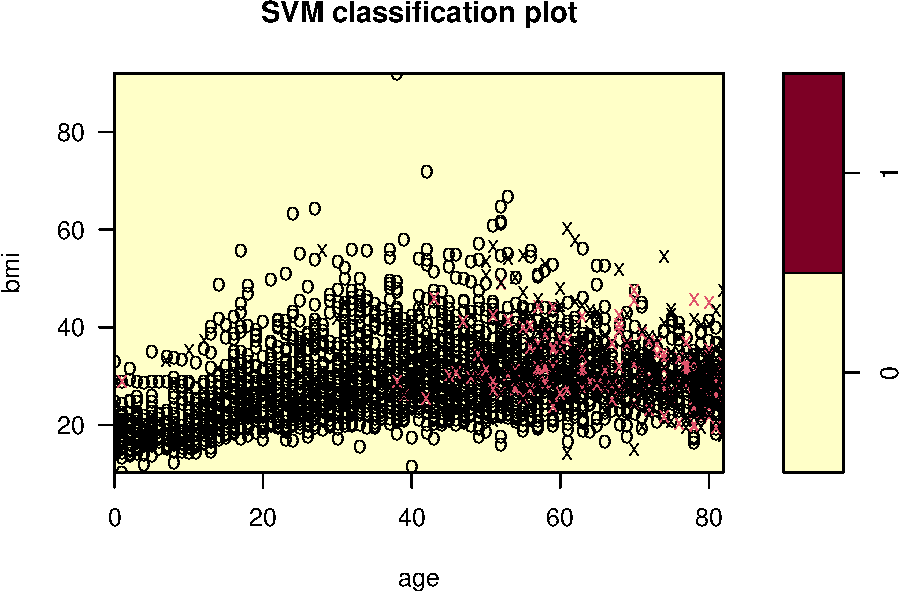
\includegraphics{sioux_mach_learn_project_files/figure-latex/unnamed-chunk-83-1.pdf}

In the following we checked the model fit with a confusion matrix with the help of the caret package's confusionMatrix() function. The following output shows an Accuracy of 94\% again. It seems that we receive the same results for the linear and the radial approach.

\begin{Shaded}
\begin{Highlighting}[]
\CommentTok{\#confusion matrix for training error}
\NormalTok{svm\_training\_prediction }\OtherTok{\textless{}{-}} \FunctionTok{predict}\NormalTok{(svm\_model\_radial, }\AttributeTok{newdata =}\NormalTok{ df\_train\_svm)}
\NormalTok{svm\_training\_error }\OtherTok{\textless{}{-}} \FunctionTok{mean}\NormalTok{(svm\_training\_prediction }\SpecialCharTok{!=}\NormalTok{ ytrain)}
\FunctionTok{confusionMatrix}\NormalTok{(svm\_training\_prediction, df\_train\_svm}\SpecialCharTok{$}\NormalTok{stroke)}
\end{Highlighting}
\end{Shaded}

\begin{verbatim}
## Confusion Matrix and Statistics
## 
##           Reference
## Prediction    0    1
##          0 3395  180
##          1    0    2
##                                          
##                Accuracy : 0.9497         
##                  95% CI : (0.942, 0.9566)
##     No Information Rate : 0.9491         
##     P-Value [Acc > NIR] : 0.459          
##                                          
##                   Kappa : 0.0207         
##                                          
##  Mcnemar's Test P-Value : <2e-16         
##                                          
##             Sensitivity : 1.00000        
##             Specificity : 0.01099        
##          Pos Pred Value : 0.94965        
##          Neg Pred Value : 1.00000        
##              Prevalence : 0.94912        
##          Detection Rate : 0.94912        
##    Detection Prevalence : 0.99944        
##       Balanced Accuracy : 0.50549        
##                                          
##        'Positive' Class : 0              
## 
\end{verbatim}

\begin{Shaded}
\begin{Highlighting}[]
\NormalTok{svm\_training\_error}
\end{Highlighting}
\end{Shaded}

\begin{verbatim}
## [1] 0.0503215
\end{verbatim}

\begin{Shaded}
\begin{Highlighting}[]
\FunctionTok{confusionMatrix}\NormalTok{(svm\_training\_prediction,df\_train\_svm}\SpecialCharTok{$}\NormalTok{stroke)}
\end{Highlighting}
\end{Shaded}

\begin{verbatim}
## Confusion Matrix and Statistics
## 
##           Reference
## Prediction    0    1
##          0 3395  180
##          1    0    2
##                                          
##                Accuracy : 0.9497         
##                  95% CI : (0.942, 0.9566)
##     No Information Rate : 0.9491         
##     P-Value [Acc > NIR] : 0.459          
##                                          
##                   Kappa : 0.0207         
##                                          
##  Mcnemar's Test P-Value : <2e-16         
##                                          
##             Sensitivity : 1.00000        
##             Specificity : 0.01099        
##          Pos Pred Value : 0.94965        
##          Neg Pred Value : 1.00000        
##              Prevalence : 0.94912        
##          Detection Rate : 0.94912        
##    Detection Prevalence : 0.99944        
##       Balanced Accuracy : 0.50549        
##                                          
##        'Positive' Class : 0              
## 
\end{verbatim}

\begin{Shaded}
\begin{Highlighting}[]
\CommentTok{\#confusion matrix for test data}
\NormalTok{svm\_prediction }\OtherTok{\textless{}{-}} \FunctionTok{predict}\NormalTok{(svm\_model\_radial, }\AttributeTok{newdata =}\NormalTok{ df\_test\_svm)}
\NormalTok{svm\_test\_error }\OtherTok{\textless{}{-}} \FunctionTok{mean}\NormalTok{(svm\_prediction }\SpecialCharTok{!=}\NormalTok{ ytest)}
\FunctionTok{confusionMatrix}\NormalTok{(svm\_prediction,df\_test\_svm}\SpecialCharTok{$}\NormalTok{stroke)}
\end{Highlighting}
\end{Shaded}

\begin{verbatim}
## Confusion Matrix and Statistics
## 
##           Reference
## Prediction    0    1
##          0 1466   67
##          1    0    0
##                                          
##                Accuracy : 0.9563         
##                  95% CI : (0.9448, 0.966)
##     No Information Rate : 0.9563         
##     P-Value [Acc > NIR] : 0.5324         
##                                          
##                   Kappa : 0              
##                                          
##  Mcnemar's Test P-Value : 7.433e-16      
##                                          
##             Sensitivity : 1.0000         
##             Specificity : 0.0000         
##          Pos Pred Value : 0.9563         
##          Neg Pred Value :    NaN         
##              Prevalence : 0.9563         
##          Detection Rate : 0.9563         
##    Detection Prevalence : 1.0000         
##       Balanced Accuracy : 0.5000         
##                                          
##        'Positive' Class : 0              
## 
\end{verbatim}

\begin{Shaded}
\begin{Highlighting}[]
\NormalTok{svm\_test\_error}
\end{Highlighting}
\end{Shaded}

\begin{verbatim}
## [1] 0.04370515
\end{verbatim}

In the following we tune the parameters for the SVM while changing C.

\begin{Shaded}
\begin{Highlighting}[]
\CommentTok{\#tune parameters for svm}
\FunctionTok{set.seed}\NormalTok{(}\DecValTok{123}\NormalTok{)}
\NormalTok{tuned\_svm }\OtherTok{\textless{}{-}} \FunctionTok{tune}\NormalTok{(svm, stroke }\SpecialCharTok{\textasciitilde{}}\NormalTok{ . , }\AttributeTok{data =}\NormalTok{ df\_train\_svm, }\AttributeTok{ranges =} \FunctionTok{list}\NormalTok{(}\AttributeTok{epsilon =} \FunctionTok{seq}\NormalTok{(}\DecValTok{0}\NormalTok{, }\DecValTok{1}\NormalTok{, }\FloatTok{0.1}\NormalTok{), }\AttributeTok{cost =} \DecValTok{2}\SpecialCharTok{\^{}}\NormalTok{(}\DecValTok{2}\SpecialCharTok{:}\DecValTok{5}\NormalTok{)))}
\NormalTok{tuned\_svm}
\end{Highlighting}
\end{Shaded}

\begin{verbatim}
## 
## Parameter tuning of 'svm':
## 
## - sampling method: 10-fold cross validation 
## 
## - best parameters:
##  epsilon cost
##        0    4
## 
## - best performance: 0.0511627
\end{verbatim}

In the following plot we see the Performance of the SVM. The darker the colour, the lower the misclassification error. Therefore, we can say, the lower values and epsilon works best for our model.

\begin{Shaded}
\begin{Highlighting}[]
\FunctionTok{plot}\NormalTok{(tuned\_svm)}
\end{Highlighting}
\end{Shaded}

\includegraphics{sioux_mach_learn_project_files/figure-latex/unnamed-chunk-87-1.pdf}

\begin{Shaded}
\begin{Highlighting}[]
\FunctionTok{summary}\NormalTok{(tuned\_svm)}
\end{Highlighting}
\end{Shaded}

\begin{verbatim}
## 
## Parameter tuning of 'svm':
## 
## - sampling method: 10-fold cross validation 
## 
## - best parameters:
##  epsilon cost
##        0    4
## 
## - best performance: 0.0511627 
## 
## - Detailed performance results:
##    epsilon cost      error  dispersion
## 1      0.0    4 0.05116270 0.009243078
## 2      0.1    4 0.05116270 0.009243078
## 3      0.2    4 0.05116270 0.009243078
## 4      0.3    4 0.05116270 0.009243078
## 5      0.4    4 0.05116270 0.009243078
## 6      0.5    4 0.05116270 0.009243078
## 7      0.6    4 0.05116270 0.009243078
## 8      0.7    4 0.05116270 0.009243078
## 9      0.8    4 0.05116270 0.009243078
## 10     0.9    4 0.05116270 0.009243078
## 11     1.0    4 0.05116270 0.009243078
## 12     0.0    8 0.05255935 0.009581009
## 13     0.1    8 0.05255935 0.009581009
## 14     0.2    8 0.05255935 0.009581009
## 15     0.3    8 0.05255935 0.009581009
## 16     0.4    8 0.05255935 0.009581009
## 17     0.5    8 0.05255935 0.009581009
## 18     0.6    8 0.05255935 0.009581009
## 19     0.7    8 0.05255935 0.009581009
## 20     0.8    8 0.05255935 0.009581009
## 21     0.9    8 0.05255935 0.009581009
## 22     1.0    8 0.05255935 0.009581009
## 23     0.0   16 0.05507253 0.011706023
## 24     0.1   16 0.05507253 0.011706023
## 25     0.2   16 0.05507253 0.011706023
## 26     0.3   16 0.05507253 0.011706023
## 27     0.4   16 0.05507253 0.011706023
## 28     0.5   16 0.05507253 0.011706023
## 29     0.6   16 0.05507253 0.011706023
## 30     0.7   16 0.05507253 0.011706023
## 31     0.8   16 0.05507253 0.011706023
## 32     0.9   16 0.05507253 0.011706023
## 33     1.0   16 0.05507253 0.011706023
## 34     0.0   32 0.05954963 0.011728863
## 35     0.1   32 0.05954963 0.011728863
## 36     0.2   32 0.05954963 0.011728863
## 37     0.3   32 0.05954963 0.011728863
## 38     0.4   32 0.05954963 0.011728863
## 39     0.5   32 0.05954963 0.011728863
## 40     0.6   32 0.05954963 0.011728863
## 41     0.7   32 0.05954963 0.011728863
## 42     0.8   32 0.05954963 0.011728863
## 43     0.9   32 0.05954963 0.011728863
## 44     1.0   32 0.05954963 0.011728863
\end{verbatim}

Now, lets choose the best model for our Data.

\begin{Shaded}
\begin{Highlighting}[]
\CommentTok{\#choose the best model based on hyperparameter }
\NormalTok{svm\_after\_tuned }\OtherTok{\textless{}{-}}\NormalTok{ tuned\_svm}\SpecialCharTok{$}\NormalTok{best.model}
\FunctionTok{summary}\NormalTok{(svm\_after\_tuned)}
\end{Highlighting}
\end{Shaded}

\begin{verbatim}
## 
## Call:
## best.tune(method = svm, train.x = stroke ~ ., data = df_train_svm, 
##     ranges = list(epsilon = seq(0, 1, 0.1), cost = 2^(2:5)))
## 
## 
## Parameters:
##    SVM-Type:  C-classification 
##  SVM-Kernel:  radial 
##        cost:  4 
## 
## Number of Support Vectors:  596
## 
##  ( 182 414 )
## 
## 
## Number of Classes:  2 
## 
## Levels: 
##  0 1
\end{verbatim}

\begin{Shaded}
\begin{Highlighting}[]
\CommentTok{\#plot the tuned SVM model}
\FunctionTok{plot}\NormalTok{(svm\_after\_tuned, }\AttributeTok{data =}\NormalTok{ df\_train\_svm, bmi }\SpecialCharTok{\textasciitilde{}}\NormalTok{ age, }\AttributeTok{slice =} \FunctionTok{list}\NormalTok{(}\AttributeTok{avg\_glucose\_level =} \DecValTok{3}\NormalTok{))}
\end{Highlighting}
\end{Shaded}

\includegraphics{sioux_mach_learn_project_files/figure-latex/unnamed-chunk-89-1.pdf}

Again, we checked the Accuracy of the model after tuning the hyperparameters with the help of the confusion matrix. As we can see, the model receives an accuracy of 95\%. Again, we receive the same results with the radial kernel as we did with the linear kernel.

\begin{Shaded}
\begin{Highlighting}[]
\CommentTok{\# Confusion matrix after tuning hyperparameters}
\NormalTok{svm\_prediction\_tuned }\OtherTok{\textless{}{-}} \FunctionTok{predict}\NormalTok{(svm\_after\_tuned, }\AttributeTok{newdata =}\NormalTok{ df\_test\_svm)}
\NormalTok{svm\_tuned\_test\_error }\OtherTok{\textless{}{-}} \FunctionTok{mean}\NormalTok{(svm\_prediction\_tuned }\SpecialCharTok{!=}\NormalTok{ ytest)}
\FunctionTok{confusionMatrix}\NormalTok{(svm\_prediction\_tuned,df\_test\_svm}\SpecialCharTok{$}\NormalTok{stroke)}
\end{Highlighting}
\end{Shaded}

\begin{verbatim}
## Confusion Matrix and Statistics
## 
##           Reference
## Prediction    0    1
##          0 1466   67
##          1    0    0
##                                          
##                Accuracy : 0.9563         
##                  95% CI : (0.9448, 0.966)
##     No Information Rate : 0.9563         
##     P-Value [Acc > NIR] : 0.5324         
##                                          
##                   Kappa : 0              
##                                          
##  Mcnemar's Test P-Value : 7.433e-16      
##                                          
##             Sensitivity : 1.0000         
##             Specificity : 0.0000         
##          Pos Pred Value : 0.9563         
##          Neg Pred Value :    NaN         
##              Prevalence : 0.9563         
##          Detection Rate : 0.9563         
##    Detection Prevalence : 1.0000         
##       Balanced Accuracy : 0.5000         
##                                          
##        'Positive' Class : 0              
## 
\end{verbatim}

\begin{Shaded}
\begin{Highlighting}[]
\NormalTok{svm\_tuned\_test\_error}
\end{Highlighting}
\end{Shaded}

\begin{verbatim}
## [1] 0.04370515
\end{verbatim}

\begin{Shaded}
\begin{Highlighting}[]
\CommentTok{\#compare the tuned prediction with the test data }
\FunctionTok{confusionMatrix}\NormalTok{(svm\_prediction\_tuned,df\_test\_svm}\SpecialCharTok{$}\NormalTok{stroke)}
\end{Highlighting}
\end{Shaded}

\begin{verbatim}
## Confusion Matrix and Statistics
## 
##           Reference
## Prediction    0    1
##          0 1466   67
##          1    0    0
##                                          
##                Accuracy : 0.9563         
##                  95% CI : (0.9448, 0.966)
##     No Information Rate : 0.9563         
##     P-Value [Acc > NIR] : 0.5324         
##                                          
##                   Kappa : 0              
##                                          
##  Mcnemar's Test P-Value : 7.433e-16      
##                                          
##             Sensitivity : 1.0000         
##             Specificity : 0.0000         
##          Pos Pred Value : 0.9563         
##          Neg Pred Value :    NaN         
##              Prevalence : 0.9563         
##          Detection Rate : 0.9563         
##    Detection Prevalence : 1.0000         
##       Balanced Accuracy : 0.5000         
##                                          
##        'Positive' Class : 0              
## 
\end{verbatim}

\hypertarget{conclusion}{%
\section{Conclusion}\label{conclusion}}

\newpage

\end{document}
